\documentclass[12pt]{amsart}

\usepackage{amsmath, amssymb, bm, MnSymbol, amsrefs}
\usepackage[hidelinks]{hyperref}
\usepackage[all]{xy}
\usepackage{diagrams}
\usepackage{enumerate}
\usepackage{graphicx}

\setlength{\textwidth}{16cm} \setlength{\textheight}{22cm}
\setlength{\oddsidemargin}{0cm} \setlength{\topmargin}{0cm}
\setlength{\evensidemargin}{0cm} \setlength{\topmargin}{0cm}

\newtheorem{theorem}{Theorem}[section]
\newtheorem{proposition}[theorem]{Proposition}
\newtheorem{lemma}[theorem]{Lemma}
\newtheorem{corollary}[theorem]{Corollary}
\newtheorem{conjecture}[theorem]{Conjecture}
\newtheorem{question}[theorem]{Question}
\theoremstyle{definition}
\newtheorem{remark}[theorem]{Remark}
\newtheorem{example}[theorem]{Example}
\newtheorem{dfn}[theorem]{Definition}
\newtheorem{property}[theorem]{Property}
\newtheorem{notation}[theorem]{Notation}
\newtheorem{exercise}[theorem]{Exercise}

\title{Linear Algebra}

\begin{document}
\maketitle

\begin{center}Dinh Huu Nguyen, Fall 2014\end{center}
\vspace{20pt}

Abstract: lecture notes for Advanced Linear Algebra at John von Neumann Institute, Vietnam, Fall 2014.

\tableofcontents
\part{Linear Algebra} Linear algebra is central to both pure and applied mathematics. We study vector spaces and linear maps between them over a field. Most of the times, this field is a general field $F$. Other times, this field is the real numbers $\mathbb{R}$.

\section{Vector Spaces}
\subsection{Basic Objects} We begin with the usual Euclidean spaces
$$\mathbb{R} = \{\text{all real numbers}\}$$
$$\mathbb{R} \times \ldots \times \mathbb{R} = \mathbb{R}^n = \{\text{all } (x_1, \dots , x_n), x_i \in \mathbb{R}\}, n \geq 2$$

Each element $(x_1, \dots , x_n)$ is called an $n$-tuple and each $x_i$ is called its $i^{\text{th}}$ component or $i^{\text{th}}$ coordinate. Like real numbers, the elements in $\mathbb{R}^n$ can be added
$$(x_1, \dots , x_n) + (y_1, \dots , y_n) = (x_1 + y_1, \dots , x_n + y_n)$$
and scaled by a real number
$$a (x_1, \dots , x_n) = (a x_1, \dots , a x_n)$$
for all $(x_1, \dots , x_n), (y_1, \dots , y_n) \in \mathbb{R}^n, a \in \mathbb{R}$. These algebraic operations impose a structure on $\mathbb{R}^n$. We consider its abstract generalization.
\dfn A vector space over a field $F$ is a set $V$ together with a binary operation $+$ and a scalar multiplication $\cdot$ that satisfy the following axioms
\begin{enumerate}[\indent 1.]
\item (closure under addition) $v + w \in V$ for any $v, w \in V$.
\item (associativity of addition) $(u + v) + w = u + (v + w)$ for all $u, v, w \in V$.
\item (commutativity of addition) $v + w = w + v$.
\item (identity element under addition) there exists an element $0 \in V$ such that $0 + v = v + 0 = v$ for all $v \in V$.
\item (inverse element under addition) there exists an element $-v$ such that $v + (-v) = -v + v = 0$ for all $v \in V$.
\item (closure under scalar multiplication) $a \cdot v \in V$ for any $a \in F$ and $v \in V$.
\item (distributivity of scalar multiplication with respect to vector addition) $a \cdot (v + w) = a \cdot v + a \cdot w$.
\item (distributivity of scalar multiplication with respect to field addition) $(a + b) \cdot v = a \cdot v + b \cdot v$.
\item (compatibility of scalar multiplication with field multiplication) $(a b) \cdot v = a \cdot (b \cdot v)$.
\item (identity element of scalar multiplication) $1 \cdot v = v$ for $1 \in F$ and any $v \in V$.
\end{enumerate}

For those who have studied abstract algebra, the first five axioms mean $V$ is a group under $+$ and the next five axioms mean $V$ is an $F$-module. The elements in $V$ are called vectors while the elements in $F$ are called scalars. We denote this vector space structure by $(V, + , \cdot_F)$ or $(V, + , \cdot)$ or $V/F$ or simply $V$. Below are some examples.

\begin{example} The set $V = \{\ast\}$ a single point over the field $\mathbb{Q}$ under the trivial $+$ and $\cdot$ is a vector space. It is called the zero vector space and denoted by $\{0\}$. The same holds when we replace $\mathbb{Q}$ with any field $F$.
\end{example}

\begin{example} The plane $\mathbb{R}^2 = \{(x, y) \text{ with } x, y \in \mathbb{R}\}$ over the field $\mathbb{R}$ under the usual operations $+$ and $\cdot$ is a vector space. More generally, the space $\mathbb{R}^n = \{(x_1, \dots ,  x_n) \text{ with } x_i \in \mathbb{R}\}$ over the field $\mathbb{R}$ under the usual operations $+$ and $\cdot$ is a vector space.
\end{example}

\begin{example}\label{} The rational plane $\mathbb{Q}^2 = \{(x, y) \text{ with } x, y \in \mathbb{Q}\}$ over the field $\mathbb{R}$ under the usual operations $+$ and $\cdot$ is not a vector space.
\end{example}

\begin{example}\label{finitesum} The set $S = \{ \sum\limits_{i=1}^{n}a_ix^i \}$ of all finite sums of length $n$ where $a_i \in \mathbb{C}$ and $x$ is an indeterminate over the field $\mathbb{C}$ under the usual operations $+$ and $\cdot$ is a vector space.
\end{example}

\begin{example}\label{mapsfromR^ntoR} We consider different classes of maps from $\mathbb{R}^n$ to $\mathbb{R}$.
\begin{enumerate}[\indent a.]
\item A map $\mathbb{R}^n \rTo^f \mathbb{R}, (x_1, \dots , x_n) \mapsto f(x_1, \dots , x_n)$ is called linear if $f(a v + b w) = a f(v) + b f(w)$ for any $a, b \in \mathbb{R}, v, w \in \mathbb{R}^n$. If we define addition $f+g$ as $(f + g)(v) = f(v) + g(v)$ and scalar multiplication as $(a \cdot f)(v) = a f(v)$ then the set $L(\mathbb{R}^n, \mathbb{R}) = \{\text{all linear maps } \mathbb{R}^n \rTo^{f} \mathbb{R}\}$ over the field $\mathbb{R}$ under $+$ and $\cdot$ is a vector space.
\item More generally, a map $\mathbb{R}^n \rTo^g \mathbb{R}, (x_1, \dots , x_n) \mapsto g(x_1, \dots , x_n)$ is called affine if $g(v) = f(v) + a$ for some linear map $f$ and some $a \in \mathbb{R}$. One can verify that this condition is equivalent to the condition $g(a v + b w) = a f(v) + b f(w)$ for any $a + b = 1$ and $v, w \in \mathbb{R}^n$. The set $M(\mathbb{R}^n, \mathbb{R}) = \{\text{all affine maps }\mathbb{R}^n \rTo^{g} \mathbb{R}\}$ over the field $\mathbb{R}$ under operations $+$ and $\cdot$ is a vector space.
\item Most generally, the set $N(\mathbb{R}^n, \mathbb{R}) = \{\text{all maps }\mathbb{R}^n \rTo^{h} \mathbb{R}\}$ over the field $\mathbb{R}$ under same operations is a vector space.
\end{enumerate}
\end{example}

One can see that $L(\mathbb{R}^n, \mathbb{R}) \subset M(\mathbb{R}^n, \mathbb{R}) \subset N(\mathbb{R}^n, \mathbb{R})$ and the operations on each subset agree with the operations from the larger set. So in a sense $L(\mathbb{R}^n, \mathbb{R})$ is a subspace of $M(\mathbb{R}^n, \mathbb{R})$ which is a subspace of $N(\mathbb{R}^n, \mathbb{R})$. Abstractly, whenever we have objects with some structure, we also consider subobjects with the same structure.
\dfn A subset $U \subset V$ of a vector space $(V, +, \cdot)$ is called a subspace if $U$ under $+$ and $\cdot$ is also a vector space over $F$.

\begin{example} In example \ref{mapsfromR^ntoR} $L(\mathbb{R}^n, \mathbb{R}) \subset M(\mathbb{R}^n, \mathbb{R}) \subset N(\mathbb{R}^n, \mathbb{R})$ as subspaces over $\mathbb{R}$. We will know more about them later.
\end{example}

\begin{example} \label{R2inR3} We can view $\mathbb{R}^2$ as a subspace $U = \{(x, y,0), x, y \in \mathbb{R}\} \subset \mathbb{R}^3$. Why isn't $U' = \{(x, y,1), x, y \in \mathbb{R}\} \subset \mathbb{R}^3$ a subspace?
\end{example}

We associate the first invariant to each vector space $V$ over a field $F$, generalizing the notion of dimension that we often speak of for $\mathbb{R}^n$.
\dfn A finite sum $\sum\limits_{i=1}^n a_iv_i = a_1v_1 + \ldots + a_n v_n$ with $a_i \in F, v_i \in V$ is called a linear combination of $v_1, \dots , v_n$. The set of all linear combinations of $v_1, \dots , v_n$ is called their span and denoted by $\text{Span}(v_1, \dots , v_n)$. If there exist $a_1, \dots , a_n$, not all zero, such that $a_1v_1 + \ldots + a_n v_n = 0$ then we say the $v_1, \dots , v_n$ are linearly dependent. Else we say they are linearly independent.

\begin{example} It is easy to verify that $(1,0), (0,1)$ are linearly independent in $\mathbb{R}^2$ while $(2, 1, 1), (0, 1, 2), (4, 5, 8)$ are linearly dependent in $\mathbb{R}^3$.
\end{example}

\begin{example} Any pair $x^i, x^j, i \neq j$ in example \ref{finitesum} are linearly independent.
\end{example}

\dfn A subset $B = \{v_i\}_{i \in I}, I$ an indexing set and $v_i \in V$, is called a basis for $V$ if $B$ is linearly independent and $\text{Span}(B) = V$.

In this course, we only consider vector spaces with finite basis $B = \{v_1, \dots , v_n\}$. By definition, every $v \in V$ can be written as a linear combination $v = \sum\limits_{i = 1}^n a_i v_i$ and such representation is unique by linear independence of $B$. The tuple $(a_1, \dots , a_n)$ is called the coordinate form of $v$. One can imagine that it has different representations and different coordinate forms in different bases.

\begin{example}\label{changeofbasis1} If we choose $B = \{(1,0),(0,1)\}$ as basis for $\mathbb{R}^2$ then $v = (3,4)$ can be written as $3(1,0) + 4(0,1)$ with coordinate form $(3,4)$. If we choose $B' = \{(0,1),(1,0)\}$ then $v = 4(0,1) + 3(1,0)$ with coordinate form $(4,3)$. If we choose $B'' = \{(1,0), (0,2)\}$ then $v = 3(1,0) + 2(0,2)$ with coordinate form $(3,2)$.
\end{example}

\begin{exercise}\label{changeofbasis2} Find the linear representation and coordinate form for $(3,4)$ in basis $B''' = \{(1/ \sqrt{2}, 1/ \sqrt{2}), (-1/ \sqrt{2}, 1/ \sqrt{2})\}$.
\end{exercise}

The previous examples show no basis is more special than the rest, only some bases are nicer for computation than others. Moreover, the order in each basis affects coordinate form representation. What is true is every vector space has a basis and all bases of $V$ have the same size. This is the first invariant we associate to each vector space $V$ over a field $F$.
\dfn We define the dimension $\dim(V/F)$ of $V/F$ as the size of any basis for $V$.

\begin{example} The vectors $e_1 = (1,0, \dots, 0), \dots , e_n = (0, \dots, 0, 1)$ form a basis for $\mathbb{R}^n$ over $\mathbb{R}$ since they are clearly linearly independent and any $(x_1, \dots , x_n)$ can be written as $x_1(1,0, \dots , 0) + \ldots + x_n(0, \dots , 1), x_i \in \mathbb{R}$. Therefore the dimension of $\mathbb{R}^n$ over $\mathbb{R}$ is $n$ as conventionally known. They do not form a basis for $\mathbb{R}^n$ over $\mathbb{Q}$.
\end{example}

\begin{example} The vectors $x, x^2, \dots , x^n$ together form a basis for our vector space $V$ over $\mathbb{C}$ in example \ref{finitesum}. Its dimension is $n$. Viewed as a vector space over $\mathbb{R}$, however $V$ has dimension $2n$ since one of its bases is $x, ix, x^2, ix^2, \dots , x^n, ix^n$.
\end{example}

\begin{example} The vector space $N$ in example \ref{mapsfromR^ntoR} does not have a finite basis. It fact, any of its bases must be uncountable. We say it has infinite dimension over $\mathbb{R}$.
\end{example}

\subsection{Inner Product} We begin this subsection by considering vector spaces over $\mathbb{R}$. If they are to enjoy multiplication $V \times V \rTo \mathbb{R}, (v, w) \mapsto v \cdot w$, we expect the following.
\dfn An inner product on a vector space $V$ over $\mathbb{R}$ is any map $V \times V \rTo^{\langle -, - \rangle} \mathbb{R}$ that satisfies the following axioms,
\begin{enumerate}[\indent 1.]
\item (symmetry) $\langle v, w \rangle = \langle w, v \rangle$.
\item (linearity) $\langle a \cdot u + b \cdot v, w \rangle = a \langle u, w \rangle + b \langle v, w \rangle$.
\item (positive definiteness) $\langle v, v \rangle \geq 0$ for all $v \in V$, with equality iff $v = 0$.
\end{enumerate}

A vector space $V$ over $\mathbb{R}$ equipped with an inner product is called an inner product space. Note that the product of two vectors is a scalar in $\mathbb{R}$.

\begin{example}\label{usualinnerproductforR^n} We can turn $\mathbb{R}^n$ into an inner product space as follows. Given two vectors $v = (x_1, \dots, x_n), w = (y_1, \dots, y_n) \in \mathbb{R}^n$ we define their inner product to be $\langle v, w \rangle = \sum\limits_{i = 1}^n x_i y_i = x_1y_1 + \ldots + x_n y_n$. One can verify that this newly minted product satisfies the above three axioms.
\begin{enumerate}[\indent a.]
\item If $v = (3,4)$ and $w = (5,6)$ in $\mathbb{R}^2$ then $\langle v, w \rangle = 3 \cdot 5 + 4 \cdot 6 = 39$
\item  If $v = (x_1, \dots, x_n)$ and $w = (y_1, \dots, y_n)$ in $\mathbb{R}^n$ where $x_i, y_i \in \{0,1\}$ then $\langle v, w \rangle$ is the number of indices $i$ where $a_i = b_i = 1$.
\item If $v = (x_1, \dots, x_n)$ then $\langle v, e_i \rangle = x_i$ its $i^{\text{th}}$ coordinate.
\end{enumerate}
\end{example}

If we look closely, we will see that any inner product $V \times V \rTo^{\langle - , - \rangle} \mathbb{R}$ is completely determined by $\langle v_i, v_j \rangle, 1 \leq i, j \leq n$ for any basis $B = \{v_1, \dots, v_n\}$ by linearity. So if we drop the requirement of positive definiteness, we can define other inner products for $V$ by setting $\langle v_i, v_j \rangle = \langle v_j, v_i \rangle = \alpha_{ij}$ (for symmetry) and extending by linearity.
\begin{align*}
V \times V & \rTo^{\langle - , - \rangle} \mathbb{R} \\
(v, w) = (\sum\limits_{i = 1}^n a_i v_i, \sum\limits_{i=1}^n b_i v_i) & \mapsto \sum\limits_{i, j} a_i b_j \alpha_{ij}
\end{align*}

\begin{example}\label{otherinnerproductforR^n} For $\mathbb{R}^n$ over $\mathbb{R}$, if we set $\langle e_i, e_j \rangle = \delta_{ij}$ then we get the inner product in example \ref{usualinnerproductforR^n}. On the other hand, if we set $\langle e_i, e_j \rangle = i + j$ then $\langle (3,4), (5,6) \rangle = \langle 3e_1 + 4e_2, 5e_1 + 6e_2 \rangle = 15\langle e_1, e_1 \rangle + (18 + 20)\langle e_1, e_2 \rangle + 24\langle e_2, e_2 \rangle = 15 \cdot 2 + 38 \cdot 3 + 24 \cdot 4 = 240$.
\end{example}

We can use this approach to define inner products for vectors space over a general $F$.
\begin{align*}
V \times V & \rTo^{\langle - , - \rangle} F\\
(v_i, v_j) & \mapsto \alpha_{ij}\\
(v_j, v_i) & \mapsto \alpha_{ij}\\
(v, w) = (\sum\limits_{i = 1}^n a_i v_i, \sum\limits_{i=1}^n b_i v_i) & \mapsto \sum\limits_{i, j} a_i b_j \alpha_{ij}
\end{align*}

\subsection{Norm} Given a vector space $V$ over $\mathbb{R}$ we want to make precise how large each vector $v \in V$ is. Of course, there are different ways to do so but they all must meet certain expectations.
\dfn A norm on $V$ over $\mathbb{R}$ is a map $V \rTo^{|| - ||} \mathbb{R}$ that satisfies,
\begin{enumerate}[\indent 1.]
\item (positive definiteness) $||v|| \geq 0$, with equality iff $v = 0$.
\item (homogeneity) $|| a \cdot v || = |a| \, || v ||$.
\item (triangle inequality) $|| v + w || \leq ||v|| + ||w||$.
\end{enumerate}

Any vector space $V$ over $\mathbb{R}$ with norm is called a normed space.

\begin{example} One obvious way to define a norm on $\mathbb{R}^n$ is $||(x_1, \dots, x_n)|| = |x_1| + \ldots + |x_n|$. This is called the 1-norm and denoted by $|| - ||_1$.
\end{example}

\begin{example} Another norm we have on $\mathbb{R}^n$ is the usual Euclidean norm $||(x_1, \dots, x_n)|| = \sqrt{x_1^2 + \ldots + x_n^2} = \sqrt{\langle v, v \rangle}$ where $\langle - , - \rangle$ is the usual inner product for $\mathbb{R}^n$. This is called the 2-norm and denoted by $|| - ||_2$. The Euclidean norm is related to the root mean square value RMS of a vector $v$ (instead of mean or mean square), defined as $\text{RMS}(v) = \sqrt{\frac{1}{n}(x_1^2 + \ldots + x_n^2)} = \frac{1}{\sqrt{n}} ||v||$. This quantity roughly tells us about the typical value of the coordinates $x_i$ with respect to $n$.
\end{example}

\begin{example} More generally we define the $p$-norm on $\mathbb{R}^n$ as $||(x_1,.., x_n)||_p = \sqrt[p]{|x_1|^p + \ldots + |x_n|^p}$ for any $1 \leq p < \infty$.
\end{example}

\begin{example} We define the $\infty$-norm on $\mathbb{R}^n$ as $||(x_1, \dots, x_n)||_{\infty} = \text{ max } \{|x_1|, \dots, |x_n|\}$.
\end{example}

\begin{exercise} Draw all the vectors of norm 1 in $\mathbb{R}^2$, where norm here is the 1-norm, the $p$-norm for $1 < p < 2$, the 2-norm, the $p$-norm for $2 < p < \infty$, and the $\infty$-norm.
\end{exercise}

We just saw that $||v||_2 = \sqrt{\langle v, v \rangle}$ where $\langle - , - \rangle$ is the usual inner product for $\mathbb{R}^n$. In general, any inner product $\langle  - , - \rangle$ on a vector space $V$ over $\mathbb{R}$ induces a map $V \rTo^{|| - ||} \mathbb{R}, v \mapsto ||v|| = \sqrt{ \langle v, v \rangle}$. Such definition easily clears the first two axioms of being a norm due to the properties of inner product. We establish a nice theorem that would imply the triangle inequality axiom.

\begin{theorem}\label{CauchySchwarz} (Cauchy-Schwarz Inequality) For all $v, w$ in an inner product space $V$ with induced norm $||-||$ we have $|\langle v, w \rangle| \leq ||v|| ||w||$. Moreover, equality holds iff $v, w$ are linearly dependent.
\end{theorem}
\begin{proof} If either $v = 0$ or $w = 0$ then inequality holds. Else consider the quadratic polynomial $p(t) = ||tv + w||^2 = \langle tv + w, tv + w \rangle = \langle v, v \rangle t^2 + 2\langle v, w \rangle t + \langle w, w \rangle$. Being a square, $p(t) \geq 0$, hence its discriminant $4\langle v, w \rangle^2 - 4\langle v, v \rangle \langle w, w \rangle \leq 0$, or $\langle v, w \rangle^2 \leq \langle v, v \rangle \langle w, w \rangle$. Equality holds iff the discriminant is 0 iff $p(t) = 0$ iff $tv + w = 0$ iff $w$ is a multiple of $v$.
\end{proof}

 Do you see why we considered such polynomial $p(t)$ as to show us exactly what we needed?
\begin{corollary}\label{triangleinequality} (Triangle Inequality) The induced norm $||-||$ from an inner product on $V$ satisfies triangle inequality $||v + w|| \leq ||v|| + ||w||$, all $v, w \in V$.
\end{corollary} 
\begin{proof} Clearly $||v + w||^2 = \langle v+w, v+w \rangle = \langle v, v \rangle + 2\langle v, w \rangle + \langle w, w \rangle = ||v||^2 + 2 \langle v, w \rangle + ||w||^2 \leq ||v||^2 + 2||v|| ||w|| + ||w||^2 = (||v|| + ||w||)^2$, from which our claim follows.
\end{proof}

Thus an inner product on $V$ induces a norm.

\subsection{Distance between Vectors} A norm in turn induces distance.
\dfn For any vectors $v, w$ in a vector space $V$ equipped with norm $||-||$ we define their distance to be $\text{dist}(v, w) = ||v - w||$.

\begin{example} All the above norms on $\mathbb{R}^n$ induce different distances between vectors in $\mathbb{R}^n$, though some of them are rather antiintuitive.
\end{example}

\subsection{Angle between Vectors} As an inner product $\langle  - , - \rangle$ induces a norm $||-||$ for $V$, we notice there is a relationship between $\langle v, w \rangle$ and $||v|| ||w||$ for any pair $v, w \in V$.
\begin{example} When $v, w$ are in the same direction, $w = a v \in V$ for some positive $a \in \mathbb{R}$ and $\langle v, w \rangle = a \langle v, v \rangle = a ||v||^2 = |a|||v|| ||v|| = ||v|| ||w||$. When $v, w$ are in opposite direction, $w = a v$ for some negative $a$ and $\langle v, w \rangle = - ||v|| ||w||$
\end{example}

Hence we suspect that the ratio $\frac{\langle v, w \rangle}{||u|| ||v||}$ bears some correlation between $v$ and $w$, perhaps how $v$ lines up against $w$.
\dfn For any nonzero vectors $v, w$ in a vector space $V$ equipped with inner product $\langle - , - \rangle$ and induced norm $||-||$ we define their correlation coefficient to be $\rho(v, w) = \frac{\langle v, w \rangle}{||v|| ||w||}$.

This correlation coefficient, viewed as a map $V \times V \rTo^{\rho} \mathbb{R}$ is surely symmetric. Its range is $[-1,1]$ by Cauchy-Schwarz inequality. Two vectors $v, w$ are said to be highly correlated if $\rho(v, w)$ is close to 1, uncorrelated if $\rho(v, w) = 0$, and highly anticorrelated if $\rho(v, w)$ is close to $-1$.

\begin{example} Consider $u = (0.1, -0.3, 1.3, -0.3, -3.3), v = (0.2, -0.4, 3.2, -0.8, -5.2), w = (1.8, -1.0, -0.6, 1.4, -0.2)$. Then $||u|| = 3.57, ||v|| = 6.17, ||w|| = 2.57, \langle u, v \rangle = 21.7, \langle u, w \rangle = -0.06, \rho(u, v) = 0.98, \rho(u, w) = -0.007$. Therefore $u$ and $v$ are more correlated than $u$ and $w$ are ($v$ is roughly twice $u$).
\end{example}

\begin{example} The set $RV((\Omega, \mathcal{F},P), (\mathbb{R},\mathcal{B}(\mathbb{R})))$ of all random variables from $(\Omega, \mathcal{F},P)$ to $(\mathbb{R},\mathcal{B}(\mathbb{R}))$ form a vector space over $\mathbb{R}$. The subset $RVF((\Omega, \mathcal{F},P), (\mathbb{R},\mathcal{B}(\mathbb{R})))$ of all random variables with finite second moment and zero mean form a subspace of $RV((\Omega, \mathcal{F},P), (\mathbb{R},\mathcal{B}(\mathbb{R})))$. If we define $\langle X, Y \rangle = \text{cov}(X, Y)$ then
\begin{enumerate}[1.]
\item (symmetry) $\langle X, Y \rangle = \langle Y, X \rangle$.
\item (linearity) $\langle aX + bY, Z \rangle = a \langle X, Z \rangle + b \langle Y, Z \rangle$.
\item (positive semidefiniteness) $\langle X, X \rangle \geq 0$ with equality iff $X$ is constant.
\end{enumerate}

Therefore, $\langle -,- \rangle$ is not quite an inner product for $RV((\Omega, \mathcal{F},P), (\mathbb{R},\mathcal{B}(\mathbb{R})))$. However, it is an inner product for the subspace $RVF((\Omega, \mathcal{F},P), (\mathbb{R},\mathcal{B}(\mathbb{R})))$ of all random variables with finite second moment and zero mean. This inner product induces the norm $||X|| = \sqrt{\langle X, X \rangle} = \sqrt{\text{cov}(X,X)} = \sqrt{\text{var}(X)} = \sigma_X$ and the correlation coefficient $\rho(X, Y) = \text{corr}(X, Y)$ in probability theory. 
\end{example}

From correlation coefficient we define angle between two vectors.
\dfn For any nonzero vectors $v, w$ in a vector space $V$ equipped with inner product $\langle - , - \rangle$, induced norm $||-||$ and correlation coefficient $\rho(-, -)$ we define their angle to be $\angle(v, w) = arccos (\rho(v, w)) = arccos \left( \frac{\langle v, w \rangle}{||v|| ||w||} \right)$.

\begin{example} The usual inner product for $\mathbb{R}^n$ and its induced norm, distance, correlation coefficient and angle give us the usual geometry for $\mathbb{R}^n, 0 \leq n \leq 3$ while generalizing to $\mathbb{R}^n, n \geq 4$. Another inner product for $\mathbb{R}^n$ would give us another, albeit strange geometry.
\end{example}

For two vectors $v, w$ in an inner product space $V$ with induced norm, correlation coefficient and angle, if $\angle(v, w) = 0^{\circ}$, i.e. they have correlation coefficient 1 then each vector is a positive multiple of the other and we say $v, w$ are aligned. If $0^{\circ} < \angle(v, w) < 90^{\circ}$, i.e. they have positive correlation coefficient then we say $v, w$ make an acute angle. If $\angle(v, w) = 90^{\circ}$, i.e. they have correlation coefficient 0 then we say $v, w$ are orthogonal and write $v \perp w$. If $90^{\circ} < \angle(v, w) < 180^{\circ}$, i.e. they have negative correlation coefficient then we say $v, w$ make an obtuse angle. Lastly, if $\angle(v, w) = 180^{\circ}$, i.e. they have correlation coefficient $-1$ then each vector is a negative multiple of the other and we say $v, w$ are antialigned. We are more interested in orthogonal vectors of norm 1 because they make excellent bases.
\dfn A vector $v$ in a normed space $V$ is called a unit vector if $||v|| = 1$.

Any vector $v \in V$ can be easily normalized and replaced by an aligned unit vector $\frac{v}{||v||}$.
\dfn A collection of vectors $\{v_1, \dots, v_n\}$ in an inner product space $V$ with induced norm are said to be orthonormal if each $v_i$ is a unit vector and $v_i \perp v_j$ for any $i \neq j$.

\begin{example}\label{orthonormalvectors} Both collections $A = \{(1,0,0), (0,1,0)\}$ and\\
$B = \{(0,0,-1), (1/\sqrt{2}, 1/\sqrt{2}, 0), (1/\sqrt{2}, -1/\sqrt{2},0)\}$ are orthonormal while\\
$C = \{(1,-1,0), (1,1,1)\}$ can be normalized into an orthonormal one.
\end{example}

We can even say a collection $\{v_1, \dots, v_n\}$ are orthonormal if $\langle v_i, v_j \rangle = \delta_{ij}$ for an inner product that does not induce norm and angle. If $v = a_1 v_1 + \ldots + a_n v_n$ is a linear combination then surely $\langle v_i, v \rangle = \langle v_i, a_1 v_1 + \ldots + a_n v_n \rangle = \sum\limits_{j=1}^n \langle v_i, a_j v_j \rangle = a_i ||v_i|| = a_i$. So taking inner product with $v_i$ picks out the $i^{\text{th}}$ coefficient in the linear combination for $v$, see example \ref{usualinnerproductforR^n}(c). It implies any orthonormal collection $\{v_1, \dots, v_n\}$ are linearly independent. This is most useful when $n = \dim(V)$ and $\{v_1, \dots, v_n\}$ form a basis for $V$.

\section{Linear Maps between Vector Spaces}

\subsection {Linear Maps}\label{linearmapmatrix} We step back from vectors within a vector space $V/F$ and consider the relationships between finite dimensional vector spaces over the same field $F$. Given two vector spaces $V/F$ and $W/F$ we would expect any map between them to respect their linear structures.
\dfn A map $V \rTo{f} W$ between two vector spaces $V, W$ over $F$ is called linear if $f(a v + b w) = a f(v) + b f(w)$ for all $v, w \in V$ and $a, b \in F$.

The set of all linear maps from $V$ to $W$ is denoted by $L(V, w)$. We can give it a vector space structure by defining addition $f+g$ where $(f+g)(v) = f(v) + g(v)$ and scalar multiplication $a \cdot f$ where $(a \cdot f)(v) = a \cdot f(v)$. That addition of linear maps is commutative and associative follows from analogous properties for additions in $V$ and in $W$.
\begin{enumerate}[\indent 1.]
\item (commutativity) $f + g = g + f$.
\item (associativity) $(f + g) + h = f + (g + h)$.
\end{enumerate}

Moreover, composition $U \rTo^f V \rTo^g W$ of two linear maps is also linear. One can verify that
\begin{enumerate}[\indent 1.]
\item (distributivity) $(f_1 + f_2) \circ g = f_1 \circ g + f_2 \circ g$ and $f \circ (g_1 + g_2) = f \circ g_1 + f \circ g_2$.
\item (associativity) $(f \circ g) \circ h = f \circ (g \circ h)$.
\end{enumerate}

\begin{example} The trivial map $V \rTo^f W, v \mapsto 0$ between any two vector spaces is certainly linear.
\end{example}

\begin{example} The map $\mathbb{R}^2 \rTo^f \mathbb{R}^3, (x, y) \mapsto (x, y,0)$ is linear. The image of $f$ is the subspace we described in example \ref{R2inR3} and this is how we often embed $\mathbb{R}^2$ into $\mathbb{R}^3$. In similar fashion can $\mathbb{R}^m$ be embedded into $\mathbb{R}^n, m \leq n$. The map $\mathbb{R}^2 \rTo^g \mathbb{R}^3, (x, y) \mapsto (x, y,1)$ however is not linear.
\end{example}

\begin{example}\label{dualofvector} Let $V$ be vector space $V$ over $F$ with basis $B = \{v_1, \dots, v_n\}$ and inner product $\langle v_i, v_j \rangle = \langle v_j, v_i \rangle = \alpha_{ij}$. For $v \in V$, the map $V \rTo^{f_v} F, w \mapsto \langle v, w \rangle$ is linear by definition of $\langle - , - \rangle$. In particular, if $\langle v_i, v_j \rangle = \delta_{ij}$ and $w = b_1v_1 + \ldots + b_nv_n$ then $f_{v_i}(w) = \langle w, v_i \rangle = b_i$ its $i^{\text{th}}$ coordinate with respect to $B$. See example \ref{usualinnerproductforR^n}(c).
\end{example}

Such maps $f_v$ in fact account for all linear maps from $V$ to $F$.

\begin{proposition}\label{duality} For any vector space $V$ over $F$ with basis $B = \{v_1, \dots, v_n\}$ and $\langle v_i, v_j \rangle = \delta_{ij}$, a map $V \rTo^f F$ is linear iff $f = f_v$ for some $v \in V$.
\end{proposition}
\begin{proof} It remains to show that for any linear map $V \rTo^f F$ and any $w = b_1 v_1 + \ldots + b_n v_n \in V$ we have $f(w) = b_1f(v_1) + \ldots + b_nf(v_n) = f_{v_1}(w) f(v_1) + \ldots + f_{v_n}(w)f(v_n) = (f(v_1)f_{v_1} + \ldots + f(v_n)f_{v_n})(w) = f_v(w)$ where $v = f(v_1)v_1 + \ldots + f(v_n)v_n$.
\end{proof}

\begin{corollary}\label{dualspace} The vector space $L(V,F)$ has dimension $n$.
\end{corollary}
\begin{proof} From the proof of the proposition, any linear map $f = f_v = f(v_1)f_{v_1} + \ldots + f(v_n) f_{v_n}$ for $v = f(v_1)v_1 + \ldots + f(v_n)v_n$. Furthermore, these $\{f_{v_1}, \dots, f_{v_n}\}$ are linearly independent, hence they form a basis for $L(V,F)$. Summarily, every basis $\{v_1, \dots, v_n\}$ for $V$ corresponds to a basis $\{f_{v_1}, \dots, f_{v_n}\}$ for $L(F, v)$. Therefore $V$ and $L(V,F)$ share the same dimension $n$.
\end{proof}

Each $f_v$ is called the dual of $v$ and denoted by $v^*$. The space $L(V,F)$ is called the dual of $V$ and denoted by $V^*$. We now look at some examples.

\begin{example} Taking average of the coordinates $\mathbb{R}^n \rTo^f \mathbb{R}, (x_1, \dots, x_n) \mapsto (x_1 + \ldots + x_n)/n$ is linear. One sees $f = f_v$ where $v = (1/n, \dots, 1/n)$.
\end{example}

\begin{example} Taking maximum of the coordinates $\mathbb{R}^n \rTo^f \mathbb{R}, (x_1, \dots, x_n) \mapsto \text{max}\{x_1, \dots, x_n\}$ is not linear. To see this, pick  $n = 2, v = (1,-1), w = (-1, 1)$. Then $f(v + w) \neq f(v) + f(w)$. Hence $f \neq f_v$ for all $v \in \mathbb{R}^n$.
\end{example} 

Corollary \ref{dualspace} tells us that $L(\mathbb{R}^n, \mathbb{R})$ has dimension $n$ and $M(\mathbb{R}^n, \mathbb{R})$ has dimension $(n+1)$ in example \ref{mapsfromR^ntoR}. While $M(\mathbb{R}^n, \mathbb{R})$ is much smaller than $N(\mathbb{R}^n, \mathbb{R})$, every continuously differentiable map $f \in N(\mathbb{R}^n, \mathbb{R})$ has a good affine approximation in $M(\mathbb{R}^n, \mathbb{R})$. Recall that if $\mathbb{R}^n \rTo^f \mathbb{R}, x \mapsto f(x)$ is a continuously differentiable then we can take the continuous partial derivatives $\frac{\partial f(x)}{\partial x_i}, i = 1, \dots, n$ and form its gradient $\nabla f(x) = (\frac{\partial f(x)}{\partial x_1}, \dots, \frac{\partial f(x)}{\partial x_n})$. The first-order Taylor approximation of $f$ near $x$ is defined as
\begin{align*}
f_{\text{aff}}(x') & = (\frac{\partial f(x)}{\partial x_1}, \dots, \frac{\partial f(x)}{\partial x_n})(x' -x)^t + f(x) \\
 & = \sum\limits_{i = 1}^{n} \frac{\partial f(x)}{\partial x_i}(x_i' - x_i) + f(x) \\
 & = \langle \nabla f(x), (x' - x)\rangle + f(x)
\end{align*}

This map $f_{\text{aff}}$ is certainly affine and gives a good approximation of $f$ when $x'$ is near $x$.

\begin{example} When $n = 1$ this is none other than the usual Taylor approximation $f_{\text{aff}}(x') = f'(x)(x' - x) + f(x)$ we often see.
\end{example}

\begin{example} Consider $\mathbb{R}^2 \rTo^f \mathbb{R}, (x_1, x_2) \mapsto e^{x_1 + x_2 -1} + e^{x_1 - x_2 -1} + e^{-x_1 -1}$. Then
$$\nabla f(x) = (e^{x_1 + x_2 -1} + e^{x_1 - x_2 -1} - e^{-x_1 -1}, e^{x_1 + x_2 -1} - e^{x_1 - x_2 -1})$$

At $(0,0)$
$$\nabla f((0,0)) = (1/e, 0)$$

Hence the first-order Taylor approximation of $f$ near $(0,0)$ is
\begin{align*}
f_{\text{aff}}(x) & = \langle \nabla f((0,0)) , x - (0,0) \rangle + f((0,0)) \\
 & = x_1/e + 3/e
\end{align*}
\end{example}

The most notable thing about a linear map $V \rTo^{f} W$ is that it is completely determined by what it does to a basis $B = \{v_1, \dots, v_n\}$ for $V$. More precisely, if we write $v = a_1 v_1 + \ldots + a_n v_n$ then $f(v) = a_1 f(v_1) + \ldots + a_n f(v_n)$ by linearity of $f$. If we also choose a basis $C = \{w_1, \dots, w_m\}$ for $W$ then we can write $f(v_i) = b_{1i} w_1 + \ldots + b_{mi}w_m = (b_{1i}, \dots, b_{mi})^t$. Hence
\begin{align*}
f(v) & = a_1 f(v_1) + \ldots + a_n f(v_n) \\
 & = a_1 (b_{11}, \dots, b_{m1})^t + \ldots + a_n(b_{1n}, \dots, b_{mn})^t \\
 & = (a_1 b_{11} + \ldots + a_n b_{1n}, \dots, a_1 b_{m1} + \ldots + a_m b_{mn})^t \\
 & = \left( \begin{array}{ccc} b_{11} & \dots & b_{1n} \\ \vdots & \vdots & \vdots \\ b_{m1} & \dots & b_{mn} \end{array} \right) (a_1, \dots, a_n)^t
\end{align*}
if we define multiplication between an $m \times n$ matrix and an $n \times 1$ matrix as such. We have used the transpose notation $t$ here without having introduced it yet. We state this in a theorem.

\begin{theorem} Any linear map $V \rTo^f W$ can be represented by a matrix $A_f$ once $V, W$ are given bases. Conversely any $m \times n$ matrix $A$ is a linear map between a vector space $V$ of dimension $n$  and a vector space $W$ of dimension $m$.
\end{theorem}
\begin{proof} It remains to show that as a map, $A(a v + a' v') = a A(v) + a' A(v)$, but this follows from definition of matrix multiplication above.
\end{proof}

When we are given a matrix $A$ without mention of domain $V$ with basis $B$ and codomain $W$ with basis $C$,  they are understood to be $F^n$ with canonical basis $\{e_1, \dots, e_n\}$ and $F^m$ with canonical basis $\{e_1, \dots, e_m\}$. Let us look at some examples.

\begin{example} The trivial map $V \rTo^0 W, v \mapsto 0$ is linear and represented by the zero matrix 0 with respect to any basis for $V$ and any basis for $W$.
\end{example}

\begin{example}\label{basisvectorsmaptocolumns} For any linear map $V \rTo^{A} W$ with respect to basis $\{v_1, \dots, v_n\}$ for $V$ and basis $\{w_1, \dots, w_m\}$ for $W$, $A(v_i)$ equals the $i^{\text{th}}$ column of $A$.
$$\left(\begin{array}{ccccc} b_{11} & \dots & b_{1i} & \dots & b_{1n} \\ \vdots & \vdots & \vdots & \vdots & \vdots \\ b_{n1} & \dots & b_{ni} & \dots & b_{nn} \end{array}\right)\left(\begin{array}{c} 0 \\ \vdots \\ 1_i \\ \vdots \\ 0 \end{array}\right) = \left(\begin{array}{c} b_{1i} \\ \vdots \\ b_{ni} \end{array}\right)$$
\end{example}

\begin{exercise}\label{} Consider an inner product space $V$ with basis $B = \{v_1, \dots, v_n\}$ and the vector space $F$ with basis $C = \{1\}$. If $\langle v_i, v_j \rangle = \langle v_j, v_i \rangle = \alpha_{ij}$ and $v = a_1v_1 + \ldots + a_nv_n$, find the matrix representation for $V \rTo^{f_v} F, w \mapsto \langle v, w \rangle$ in example \ref{dualofvector} with respect to these bases.
\end{exercise}

\begin{example}\label{changeofbasismatrix} (Change of basis matrix) The identity map $V \rTo^{id} V, v \mapsto v$ is linear. If we choose a basis $B = \{v_1, \dots, v_n\}$ for both domain and codomain then $id(v_i) = v_i = 0v_1 + \ldots + 1v_i + \ldots + 0v_n$ and $id$ is represented by the identity matrix $I$. On the other hand, if we choose a different basis $B' = \{v_1', \dots, v_n'\}$ for codomain then $id(v_i) = v_i = b_{1i}v_1' + \ldots + b_{ni}v_n'$. Hence $id$ is represented by the matrix $(b_{ij})$ and not $I$. We call this matrix the change of basis matrix and denote it by $A_{BB'}$. Moreover, the identity map going in the opposite direction is represented by the change of basis matrix $A_{B'B}$. Since composition of these two identity maps is represented by the identity matrix $I$, it follows that $A_{BB'} A_{B'B} = A_{B'B}A_{BB'} = I$.
\end{example}

\begin{example} Conversely, the identity matrix $I$ with respect to certain bases for domain and codomain may not represent the identity map. Consider the linear map
$$\mathbb{R}^2 \rTo^f \mathbb{R}^2, (1, 0) \mapsto (1, 0), (0, 1) \mapsto (0, 2)$$

If we choose basis $B = \{e_1, e_2\}$ for both domain and codomain then $(1,0), (0,1), (0,2)$ have coordinates form $\left( \begin{array}{c} 1 \\ 0 \end{array}\right), \left( \begin{array}{c} 0 \\ 1 \end{array}\right), \left( \begin{array}{c} 0 \\ 2 \end{array}\right)$ and the matrix representation for $f$ with respect to this basis is
\begin{align*}
\mathbb{R}^2 & \rTo^{\left( \begin{array}{cc} 1 & 0 \\ 0 & 2 \end{array}\right)} \mathbb{R}^2 \\
\left( \begin{array}{c} 1 \\ 0 \end{array}\right) & \mapsto \left( \begin{array}{c} 1 \\ 0 \end{array}\right) \\ \left( \begin{array}{c} 0 \\ 1 \end{array}\right) & \mapsto \left( \begin{array}{c} 0 \\ 2 \end{array}\right)
\end{align*}

However, if we choose basis $B = \{e_1, e_2\}$ for domain and basis $C = \{e_1, 2e_2\}$ for codomain then $(1,0), (0,2)$ have coordinate forms $\left( \begin{array}{c} 1 \\ 0 \end{array}\right), \left( \begin{array}{c} 0 \\ 1 \end{array}\right)$ and the matrix representation for $f$ with respect to these bases is
\begin{align*}
\mathbb{R}^2 & \rTo{\left(\begin{array}{cc} 1 & 0 \\ 0 & 1 \end{array}\right)} \mathbb{R}^2 \\
\left( \begin{array}{c} 1 \\ 0 \end{array}\right) & \mapsto \left( \begin{array}{c} 1 \\ 0 \end{array}\right) \\
\left( \begin{array}{c} 0 \\ 1 \end{array}\right) & \mapsto \left( \begin{array}{c} 0 \\ 1 \end{array}\right)
\end{align*}
\end{example}

\begin{example}\label{changeofbasisforvectors} (Change of basis for vectors) We continue with example \ref{changeofbasismatrix}. For a vector $v = a_1v_1 + \ldots + a_nv_n$ with coordinate form $(a_1, \dots, a_n)$ with respect to $B$, we have
\begin{align*}
v & = a_1v_1 + \ldots + a_n v_n \\
 & = a_1(b_{11}v_1' + \ldots + b_{n1}v_n') + \ldots + a_n(b_{1n}v_1' + \ldots + b_{nn}v_n') \\
 & = (a_1b_{11} + \ldots + a_n b_{1n})v_1' + \ldots + (a_1 b_{n1} + \ldots + a_n b_{nn})v_n'
\end{align*}

Hence its new coordinate form with respect to $B'$ is
$$(a_1 b_{11} + \ldots + a_n b_{1n}, \dots, a_1b_{n1} + \ldots + a_n b_{nn})^t = A_{BB'}(a_1, \dots, a_n)^t$$
\end{example}

\begin{exercise}\label{} Compute the change of basis matrix $A_{B''B'''}$ when we move from basis $B''$ in example \ref{changeofbasis1} to basis $B'''$ in exercise \ref{changeofbasis2}. Use it to compute coordinate form for $(3,4)$ with respect to $B'''$ and compare it with the result there.
\end{exercise}

\begin{example}\label{reflection} Reflection across any line in the plane $\mathbb{R}^2$ with the usual inner product is linear. If we choose an orthonormal basis $\{u_1, u_2\}$ such that $r(u_1) = u_2$ and $r(u_2) = u_1$ then clearly it is represented as $\left( \begin{array}{cc} 0 & 1\\ 1 & 0 \end{array} \right)$. Similarly, reflection across $u_1$ is linear and represented by the matrix $\left( \begin{array}{cc} 1 & 0 \\ 0 & -1 \end{array} \right)$ while projection onto $u_1$ is represented by $\left( \begin{array}{cc} 1 & 0 \\ 0 & 0 \end{array} \right)$.
\end{example}

\subsection{Kernel, Nullity, Image, Rank} The first thing we look at in each linear map $V \rTo^f W$ is what it annihilates in $V$ and what it covers in $W$.
\dfn For any linear map $V \rTo^f W$ we define $\ker(f) = \{v \in V \text{ such that } f(v) = 0\}$ and $\text{im}(f) = \{w \in W \text{ such that } w = f(v) \text{ for some } v \in V\}$.

One can verify that $\ker(f)$ is a subspace of $V$ and $\text{im}(f)$ is a subspace of $W$. We say $f$ is injective if $\ker(f) = \{0\}$, $f$ is surjective if $\text{im}(f) = W$, and $f$ is bijective if it is both injective and surjective.
\dfn For any linear map $V \rTo^f W$ we define $\text{nullity}(f) = \dim(\ker(f))$, called the nullity of $f$. We define $\text{rank}(f) = \dim(\text{im}(f))$, called the rank of $f$.

Clearly $f$ is injective iff $\text{nullity}(f) = 0$ and $f$ is surjective iff $\text{rank}(f) = \dim(W)$. Furthermore, if $\{v_1, \dots, v_k\}$ is a basis for $\ker(f)$ then it can be completed to a basis $\{v_1, \dots, v_k, v_{k+1}, \dots, v_n\}$ for $V$. Write any $V \owns v = a_1v_1 + \ldots + a_kv_k + a_{k+1}v_{k+1} + \ldots + a_nv_n$ then $f(v) = a_1f(v_1) + \ldots + a_kf(v_k) + a_{k+1}f(v_{k+1}) + \ldots + a_nf(v_n) = a_{k+1}f(v_{k+1}) + \ldots + a_nf(v_n)$. Therefore $\text{im}(f) = \text{Span}(f(v_{k+1}), \dots, f(v_n))$. While $\dim(\ker(f)) = k$, we see $\dim(\text{im}(f)) \leq n-k$. Equality follows from the following theorem.

\begin{theorem}\label{ranknullity} (Rank-Nullity) If $V \rTo^f W$ is a linear map then $\dim(V) = \text{ nullity}(f) + \text{ rank}(f)$.
\end{theorem}
\begin{proof} It remains to show $\{f(v_{k+1}), \dots, f(v_n)\}$ are linearly independent and thus form a basis for $\text{im}(f)$. Suppose $b_{k+1}f(v_{k+1}) + \ldots + b_nf(v_n) = 0$ for some $b_{k+1}, \dots, b_n \in F$, then $f(b_{k+1}v_{k+1} + \ldots + b_nv_n) = 0$. So $b_{k+1}v_{k+1} + \ldots + b_nv_n \in \ker(f)$ and we can write $b_{k+1}v_{k+1} + \ldots + b_nv_n = b_1v_1 + \ldots + b_kv_k$ for some $b_1, \dots, b_k \in F$. Since the $v_i$ form a basis for $V$, the $b_i$ must all be 0. In particular, $b_{k+1} = \dots = b_n = 0$.
\end{proof}

\begin{example} The zero map $V \rTo^0 W$ has $\text{nullity}(0) = \dim(V)$ and $\text{rank}(0) = 0$ while for $\lambda \neq 0$ scaling $V \rTo^{\lambda} V$ has $\text{nullity}(\lambda, \dots , \lambda) = 0$ and $\text{rank}(\lambda, \dots , \lambda) = \dim(V)$.
\end{example}

\begin{example} Reflections in example \ref{reflection} has nullity 0 and rank 2. On the other hand, projection onto $u_1$ has nullity 1 and rank 1. In general, if $\{u_1, \dots, u_k\}$ are linearly independent in $V$ then projection onto $\text{Span}(u_1, \dots, u_k)$ has $\text{rank} = k$ and $\text{nullity} = \dim(V) - k$.
\end{example}

If we view each $m \times n$ matrix $A$ as a linear map $F^n \rTo^{A} F^m$ then from example \ref{basisvectorsmaptocolumns} and theorem \ref{ranknullity}, $n-k$ of its columns will form a basis for its image while the other $k$ columns are linearly dependent upon those. Looking closely at columns of a matrix reveals information about that matrix.

\begin{example}\label{} The matrix $\left(\begin{array}{ccc} 1 & 2 & 5 \\ -1 & 0 & -1\\ 2 & -1 & 0 \\ 0 & 1 & 2 \end{array}\right)$ has rank 2 and nullity 1. It is neither injective nor surjective.
\end{example}

If linear map $V \rTo^f W$ is bijective then its inverse $W \rTo^{f^{-1}} V, w \mapsto v$ the unique element in $V$ such that $f(v) = w$ is also linear. We call such $f$ an isomorphism and say $V$ and $W$ are isomorphic. If $A_f$ is the matrix representation for $f$ with respect to some bases for $V$ and $W$ and $A_{f^{-1}}$ the matrix representation for $f^{-1}$ then surely $A_f A_{f^{-1}} = A_{f^{-1}} A_f = I$. Moreover, $\text{nullity}(f) = \text{nullity}(f^{-1}) = 0$ and d$\text{im}(V) = \text{rank}(f) = \text{rank}(f^{-1}) = \text{dim}(W)$ in that case.

\begin{example}\label{} The identity map $V \rTo^{id} V$ in example \ref{changeofbasismatrix} is an isomorphism. With basis $B$ for domain $V$ and basis $B'$ for codomain $V$, it has matrix representation $A_{BB'}$ and its inverse has matrix representation $A_{B'B}$ with $A_{BB'} A_{B'B} = A_{B'B} A_{BB'} = I$.
\end{example}

\begin{example}\label{} The association $V \rTo L(V,F), v \mapsto f_v$ in example \ref{dualofvector} is an isomorphism.
\end{example}

\begin{exercise}\label{} If $V \rTo^f W$ is a bijective linear map, show that its inverse $W \rTo^{f^{-1}} V, w \mapsto v$ the unique element in $V$ such that $f(v) = w$ is also linear.
\end{exercise}

\begin{exercise}\label{} Show that
\begin{enumerate}[\indent a.]
\item If $V$ and $W$ have the same dimension over $F$ then they are isomorphic.
\item If $V$ and $W$ have different dimensions over $F$ then they are not isomorphic.
\end{enumerate}
\end{exercise}

We end this subsection with a look at what happens to a linear map and its matrix representations with respect to different bases.

\begin{theorem}\label{changeofbasisforlinearmaps} (Change of Basis for Linear Maps) If $V \rTo^f W$ is a linear map with matrix presentation $A_f$ with respect to bases $B, C$ for $V, W$ and with matrix representation $A_f'$ with respect to bases $B', C'$ for $V, W$ then $A_f' = A_{CC'} A_f A_{BB'}^{-1}$ where $A_{BB'}$ and $A_{CC'}$ are the change of basis matrices.
\end{theorem}
\begin{proof} It follows immediately from the following commutative diagram of maps and the commutative diagram of their matrix representations with respect to different bases.
\begin{diagram}
V & \rTo^f & W & & & V & \rTo^{A_f} & W \\
\dTo^{id_V} & & \dTo_{id_W} & & & \dTo^{A_{BB'}} & & \dTo_{A_{CC'}} \\
V & \rTo_f & W & & & V & \rTo_{A_f'} & W
\end{diagram}
\end{proof}

When $W = V$ and $C' = B'$, the theorem says $A_f' = A_{BB'}A_fA_{BB'}^{-1}$ which is often written as $A_f' = UA_f U^{-1}$ in literature.

\section{Matrices} As any linear map between vector spaces over $F$ with fixed bases is represented by a matrix, we study matrices more closely. First goes a formal definition of matrix.
\dfn A matrix $M$ is a rectangular array of $(a_{ij})_{m \times n}$ of $m$ rows and $n$ columns, where each entry $a_{ij}$ in the $i^{\text{th}}$ row and $j^{\text{th}}$ column is an element in $F$. We denote the set of all $m \times n$ matrices over $F$ by $M(m, n,F)$.

\begin{example} We have
\begin{enumerate}[\indent 1.]
\item $\left(\begin{array}{c} 1/2 \\ 2 \\ 2/3 \end{array}\right) \in M(3,1, \mathbb{Q}) \text{ with } a_{3,1} = 2/3$
\item $M = \left(\begin{array}{cc} sin(\pi/10) & cos(\pi/10) \end{array}\right) \in M(1, 2, \mathbb{R}) \text{ with } a_{1,2} = cos(\pi/10)$
\item $M = \left(\begin{array}{ccc} i & e & 1 \\ \pi & 0 & 1/2 \\ ln5 & 1 & 3 \end{array}\right) \in M(3, \mathbb{C}) \text{ with } a_{2,2} = 0$
\end{enumerate}
\end{example}

Below are what we can do with matrices.

\subsection{Partition} We can  partition a matrix into submatrices. This will be useful later when we multiply matrices by blocks without fretting too much about entries.

\begin{example}\label{} If $A \in M(n, F)$ then it can be partitioned into blocks $A_{4 \times 5} = \left(\begin{array}{cc} A_{3 \times 3} & A_{3 \times 2} \\ A_{1 \times 3} & A_{1 \times 2} \end{array}\right)$. 
\end{example}

\begin{example}\label{} If $A \in M(4,5,F)$ and $B \in M(r+s, 4, F)$ then they can be partitioned into blocks for multiplication as follows
$$\left(\begin{array}{cc} B_{r \times 3} & B_{r \times 1} \\ B_{s \times 3} & B_{s \times 1} \end{array}\right) \left(\begin{array}{cc} A_{3 \times 3} & A_{3 \times 2} \\ A_{1 \times 3} & A_{1 \times 2} \end{array}\right) = \left(\begin{array}{cc} B_{r \times 3}A_{3 \times 3} + B_{r \times 1}A_{1 \times 3} & B_{r \times 3}A_{3 \times 2} + B_{r \times 1}A_{1 \times 2} \\ B_{s \times 3}A_{3 \times 3} + B_{s \times 1}A_{1 \times 3} & B_{s \times 3}A_{3 \times 2} + B_{s \times 1}A_{1 \times 2} \end{array}\right)$$.
\end{example}

\subsection{Addition} As the set $L(V, w)$ of all linear maps between $V$ and $W$ can be given a vector space structure, so can their matrix representations $M(m, n,F)$ with respect to some fixed bases.
\dfn For $A = (a_{ij}), B = (b_{ij}) \in M(m, n,F)$ we define $A + B = (c_{ij}) \in M(m, n,F)$ where $c_{ij} = a_{ij} + b_{ij}$.

\begin{example} $\left( \begin{array}{ccc} 1 & 0 & 2\\ 0 & 1 & -1 \end{array} \right) + \left( \begin{array}{ccc} 1 & 3 & 0 \\ 0 & -1 & -2 \end{array} \right) = \left( \begin{array}{ccc} 2 & 3 & 2 \\ 0 & 0 & -3 \end{array} \right)$.
\end{example}.

Addition of matrices $A + B$ clearly corresponds to addition of linear maps $V \rTo^{f_A + f_B} W$. Thus it enjoys commutativity and associativity as well.
\begin{enumerate}[\indent 1.]
\item (commutativity) $A + B = B + A$.
\item (associativity) $(A + B) + C = A + (B + C)$.
\end{enumerate}

\subsection{Multiplication} Next question is how to define scalar multiplication $a \cdot A_f$ to represent the linear map $a \cdot f$. If we represent scaling by $a$ by the matrix $(a, \dots, a)$ then we are looking at how to define the product $(a, \dots, a) A$ to represent the composition $U \rTo^f V \rTo^{a} V$. More generally, if $U \rTo^f V \rTo^g W$ are represented by $A, B$ with respect to some chosen basses for $U, v, w$ then we must define the right product $BA$ to represent $gf$. Here is the picture.
\begin{diagram}
U & \rTo^f & V & & U & \rTo^A & V & & U & \rTo^A & V \\
    & \rdTo^{gf} & \dTo^g & & & \rdTo^C & \dTo^B & & & \rdTo^{BA} & \dTo^B \\
    & & W & & & & W & & & & W
\end{diagram}

\dfn For $A = (a_{ij}) \in M(m, n, F)$ and $B = (b_{ij}) \in M(l, m,F)$ we define $BA = (c_{ij}) \in M(l, n, F)$ where $c_{ij} = a_{1j}b_{i1} + a_{2j}b_{i2} + \ldots + a_{mj}b_{im} = \sum\limits_{k=1}^{m} a_{kj}b_{ik}$ is the inner product of $i^{\text{th}}$ row of $B$ and $j^{\text{th}}$ column of $A$.

\begin{proposition} Consider $U, V, W$ over $F$ with dimensions $n, m, l$ and bases $\{u_1, \dots , u_n\}$, $\{v_1, \dots, v_m\}$, $\{w_1, \dots, w_l\}$. If $U \rTo{f} V$ is represented by $A = (a_{ij}) \in M(m, n,F)$ and $V \rTo^{g} W$ is represented by $B = (b_{ij}) \in M(l, m, F)$ then $U \rTo^{gf} W$ is represented by $BA$.
\end{proposition}
\begin{proof} We write out $A = \left(\begin{array}{ccc} a_{11} & \dots & a_{1n} \\ \vdots & & \vdots \\ a_{m1} & \dots & a_{mn} \end{array}\right), B = \left(\begin{array}{ccc} b_{11} & \dots & b_{1m} \\ \vdots & & \vdots \\ b_{l1} & \dots & b_{lm} \end{array}\right)$. Then
\begin{align*}
f(u_1) & = A(1,0, \dots , 0)^t = (a_{11}, \dots , a_{m1})^t = a_{11}v_1 + \ldots + a_{m1}v_m \\
 & \vdots \\
f(u_n) & = A(0, \dots , 0, 1)^t = (a_{1n}, \dots , a_{mn})^t = a_{1n}v_1 + \ldots + a_{mn}v_m \\
gf(u_1) & = a_{11}B(v_1) + \ldots + a_{m1}B(v_m) = a_{11}(b_{11}, \dots , b_{l1})^t + \ldots + a_{m1}(b_{1m}, \dots , b_{lm})^t \\
 & \vdots \\
gf(u_n) & = a_{1n}B(v_1) + \ldots + a_{mn}B(v_m) = a_{1n}(b_{11}, \dots , b_{l1})^t + \ldots + a_{mn}(b_{1m}, \dots , b_{lm})^t
\end{align*}

Hence $gf$ is represented by $\left(\begin{array}{ccc} a_{11}b_{11} + \ldots + a_{m1}b_{1m} & \dots & a_{1n}b_{11} + \ldots + a_{mn}b_{1m} \\ \vdots & & \vdots \\ a_{11}b_{l1} + \ldots + a_{m1}b_{lm} & \dots & a_{1n}b_{l1} + \ldots + a_{mn}b_{lm} \end{array}\right)$ which is precisely $BA$.
\end{proof}

Note that the number of columns of $A$ must equal the number of rows of $B$. This definition agrees with our earlier one in \ref{linearmapmatrix}.

\begin{example} $\left(\begin{array}{cccc} 1 & 4 & 2 & 0 \\ 2 & 1 & 5 & 6 \end{array}\right) \left(\begin{array}{ccc} 2 & 1 & 3 \\ 3 & 0 & 1 \\ 4 & 0 & 5 \\ 1 & 2 & 0 \end{array}\right) = C_{2 \times 3}$ where $c_{21} = 2 \cdot 2 + 1 \cdot 3 + 5 \cdot 4 + 6 \cdot 1 = 33$
\end{example}

As a special case we define scalar multiplication as $a A = \left(\begin{array}{ccc} a & \dots & 0 \\ \vdots & a & \vdots \\ 0 & \dots & a \end{array}\right)A$.

\begin{example} $5\left(\begin{array}{ccc} 2 & 1 & 3 \\ 3 & 0 & 1 \\ 4 & 0 & 5 \\ 1 & 2 & 0 \end{array}\right) = \left(\begin{array}{cccc} 5 & 0 & 0 & 0 \\ 0 & 5 & 0 & 0 \\ 0 & 0 & 5 & 0 \\ 0 & 0 & 0 & 5\end{array}\right)\left(\begin{array}{ccc} 2 & 1 & 3 \\ 3 & 0 & 1 \\ 4 & 0 & 5 \\ 1 & 2 & 0 \end{array}\right) = \left(\begin{array}{ccc} 10 & 5 & 15 \\ 15 & 0 & 5 \\ 20 & 0 & 25 \\ 5 & 10 & 0 \end{array}\right)$
\end{example}

This scalar multiplication together with matrix addition turn $M(m, n, F)$ into a vector space over $F$, just as $L(F^n,F^m)$ is a vector space over $F$. More is true.

\begin{theorem}\label{} For $F^n$ and $F^m$ with bases $\{e_1, \dots , e_n\}$ and $\{e_1, \dots , e_m\}$, the linear maps $(L(F^n, F^m), + , \cdot) \pile{\rTo^{\phi} \\ \lTo_{\varphi}} (M(m, n,F), + , \cdot), f \mapsto A_f, A \leftmapsto A$ are inverses of each other.
\end{theorem}
\begin{proof} This is obvious.
\end{proof}

\begin{corollary}\label{} The vector space $L(F^n,F^m)$ has dimension $mn$.
\end{corollary}
\begin{proof} The collection $\{E_{ij} = (1_{ij}), 1 \leq i \leq m, 1 \leq j \leq n\}$ form a basis for $M(m, n,F)$.
\end{proof}

It follows from analogous properties for composition and addition of linear maps that
\begin{enumerate}[\indent 1.]
\item (associativity) $(AB)C = A(BC)$
\item (distributivity) $A(B + C) = AB + AC$ and $(A + B)C = AC + BC$
\item (identity element) $I_{m \times m} A_{m \times n} = A_{m \times n}I_{n \times n} = A$ for all $A_{m \times n}$ (best when $m = n$)
\item (scalar multiplication) $a A = A a$
\end{enumerate}

If $m = n$ then (3) and (4) mean commutativity $(aI_{m \times m})A_{m \times m} = A_{m \times m}(aI_{m \times m})$ for all $a \in F$ and $I, A \in M(m, F)$. Here are a few more examples to illuminate matrix multiplication.

\begin{example} One can see $\left(\begin{array}{cc} 0 & 1 \\ 1 & 0 \end{array}\right) \left(\begin{array}{cc} 1 & 0 \\ 0 & 0 \end{array}\right) \neq \left(\begin{array}{cc} 1 & 0 \\ 0 & 0 \end{array}\right) \left(\begin{array}{cc} 0 & 1 \\ 1 & 0 \end{array}\right)$ through direct multiplication or through geometry in $\mathbb{R}^2$. Matrix multiplication is not commutative in general.
\end{example}

\begin{example} Matrix multiplication fails to cancel
$$\left(\begin{array}{cc} 1 & 0 \\ 0 & 0 \end{array}\right) \left(\begin{array}{c} 3 \\  1 \end{array}\right) = \left(\begin{array}{cc} 1 & 0 \\ 0 & 0 \end{array}\right) \left(\begin{array}{c} 3 \\  2 \end{array}\right) = \left(\begin{array}{c} 3 \\  0 \end{array}\right)$$
but clearly
$$\left(\begin{array}{c} 3 \\  1 \end{array}\right) \neq \left(\begin{array}{c} 3 \\  2 \end{array}\right)$$
\end{example}

\begin{example} Matrix multiplication has zero divisors $\left(\begin{array}{cc} 1 & 0 \\ 0 & 0 \end{array}\right) \left(\begin{array}{cc} 0 & 0 \\ 0 & 1 \end{array}\right) = \left(\begin{array}{cc} 0 & 0 \\ 0 & 0 \end{array}\right)$.
\end{example}

\begin{example} Matrix multiplication has idempotents $\left(\begin{array}{cc} 1 & 0 \\ 0 & 0 \end{array}\right) \left(\begin{array}{cc} 1 & 0 \\ 0 & 0 \end{array}\right) = \left(\begin{array}{cc} 1 & 0 \\ 0 & 0 \end{array}\right)$.
\end{example}

\begin{example} Given $a_1, \dots , a_k \in F$ and $A_1, \dots , A_k \in M(m, n,F)$ we can form a linear combination $a_1 A_1 + \ldots + a_k A_k \in M(m, n,F)$.
\end{example}

\begin{example} Given a polynomial such as $p(x) = x^2 + 2x + 3 \in \mathbb{R}[x]$, we can view it as map $\mathbb{R} \rTo^{p(x)} \mathbb{R}, 4 \mapsto 4^2 + 2 \cdot 4 + 3 = 27$. Now we can also view it as map $M(n, \mathbb{R}) \rTo^{p(x)} M(n, \mathbb{R}), A \mapsto A^2 + 2 \cdot A + 3$.
\end{example}

\subsection{Transposition} Next we attribute to each matrix $A \in M(m, n, F)$ a companion, it helps us develop matrix theory.
\dfn For $A = (a_{ij}) \in M(m, n, F)$, we define its transpose $A^t = (b_{ij}) \in M(n, m, F)$ where $b_{ij} = a_{ji}$.

\begin{proposition} Transposition has the following properties
\begin{enumerate}[\indent 1.]
\item $(A^t)^t = A$.
\item $(A + B)^t = A^t + B^t$.
\item $(a A)^t = a A^t$.
\item $(AB)^t = B^t A^t$.
\end{enumerate}
\end{proposition}
\begin{proof} Straightforward.
\end{proof}

Can you interpret these properties in terms of behavior of the associated linear maps? Noteworthy is the fact that if a linear map $V \rTo^f W$ is represented by $A \in M(m, n, F)$ with respect to basis $\{v_1, \dots , v_n\}$ for $V$ and basis $\{w_1, \dots , w_m\}$ for $W$ then its dual $W^* \rTo^{f^*} V^*$ is represented by $A^t \in M(n, m, F)$ with respect to basis $\{w_1^*, \dots , w_m^*\}$ for $W^*$ and basis $\{v_1^*, \dots , v_n^*\}$ for $V^*$.

\begin{example} $\left(\begin{array}{ccc} 2 & 1 & 4 \\  3 & 4 & 1 \\ 5 & 3 & 1 \end{array}\right)^t = \left(\begin{array}{ccc} 2 & 3 & 5 \\  1 & 4 & 3 \\ 4 & 1 & 1 \end{array}\right)$
\end{example}

\begin{example} $\left(\begin{array}{ccc} 2 & 1 & 7 \end{array}\right)^t = \left(\begin{array}{c} 2 \\ 1 \\ 7\end{array}\right)$
\end{example}

\subsection{Some Matrices} We use transposition to describe some interesting classes of matrices.

\subsubsection{Orthogonal Matrices} The first class is orthogonal matrices.
\dfn A matrix $A \in M(m, n,F)$ is called orthogonal (or more descriptively orthonormal) if $A^tA = I_n$.

It follows that if we consider the $i^{\text{th}}$ column as coordinate form of vector $v_i \in F^m$ with respect to canonical basis $\{e_1, \dots , e_m\}$ and inner product $\langle e_i, e_j \rangle = \delta_{ij}$ then $\langle v_i, v_j \rangle = \delta_{ij}$. Hence $\{v_1, \dots, v_n\}$ are an orthonormal collection of vectors in $F^m$, recall the discussion after example \ref{orthonormalvectors}. It follows that these $v_i$ are linearly independent and $m \geq n$.

\subsubsection{Triangular Matrices} The second class is triangular matrices.
\dfn A matrix $A \in M(n, F)$ is called lower triangular if all entries above the diagonal are zero, i.e. $a_{ij} = 0$ for all $i < j$. A matrix $A \in M(n, F)$ is called upper triangular if $a_{ij} = 0$ for all $i > j$. And if $a_{11} = \dots = a_{nn} = 1$ then it is called unit lower triangular or unit upper triangular.

\begin{example} We have $A = \left(\begin{array}{ccc} 4 & 0 & 0 \\ 5 & 2 & 0 \\ 3 & 6 & 1 \end{array}\right)$ is lower triangular and $A = \left(\begin{array}{ccc} 4 & 0 & 3 \\ 0 & 2 & 5 \\ 0 & 0 & 1 \end{array}\right)$ is upper triangular.
\end{example}

By definition, a matrix $A$ is lower triangular iff $A^t$ is upper triangular and vice versa, while it is both lower triangular and upper triangular iff all of its nondiagonal entries are zero. 
\dfn A matrix $A \in M(n, F)$ is called diagonal if $a_{ij} = 0$ whenever $i \neq j$.

\begin{example} These matrices are all diagonal,
$$A = \left(\begin{array}{ccc} 4 & 0 & 0 \\ 0 & 2 & 0 \\ 0 & 0 & 1 \end{array}\right) \text{ and } A^n = \left(\begin{array}{ccc} 4^n & 0 & 0 \\ \vdots & 2^n & \vdots \\ 0 & \dots & 1^n \end{array}\right)^n$$
$$B = \left(\begin{array}{ccc} 4 & 0 & 0 \\ 0 & 2 & 0 \\ 0 & 0 &1 \end{array}\right) \text{ and } B^{-1} = \left(\begin{array}{ccc} 1/4 & 0 & 0 \\ 0 & 1/2 & 0\\ 0 & 0 &1 \end{array}\right)$$
\end{example}

\begin{example}\label{} One can verify that if $A = (a_{11}, \dots , a_{nn}) \in M(n, F)$ is a diagonal matrix and $M \in M(n, F)$ is any matrix then $AM$ is the matrix whose $i^{\text{th}}$ row is the $i^{\text{th}}$ row of $A$ multiplied by $a_{ii}$.
\end{example}

We denote the set of all lower triangular matrices, upper triangular matrices and diagonal matrices as $L(n,F), U(n,F), D(n,F)$. Each set is closed under addition, multiplication and inverse. For example, if $A, B \in L(n,F)$ then $AB \in L(n,F)$. Or if $A \in U(n,F)$ is invertible then $A^{-1} \in U(n,F)$.

\subsubsection{Symmetric Matrices} Another class of matrices that transposition helps describe is symmetric matrices.

\dfn A square matrix $A \in M(n, F)$ is called symmetric if $A = A^t$, or equivalently if $a_{ij} = a_{ji}$ for all $i, j$.

\begin{example} We have
\begin{enumerate}[\indent a.]
\item $A = \left(\begin{array}{ccc} 0 & 4 & 1\\ 4 & 1 & 3 \\ 1 & 3 & 2 \end{array}\right)$ is symmetric.
\item Every diagonal matrix is symmetric while other triangular matrices are not. Draw a Venn's diagram of $L(n,F), U(n,F), D(n,F), S(n,F)$.
\end{enumerate}
\end{example}

The set of all symmetric matrices is denoted by $S(n,F)$. It is closed under addition and inverse, but not under multiplication. One sure source for symmetric matrices is taking inner products of vectors. If $u = a_1 v_1 + \ldots + a_n v_n$ and $w = b_1 v_1 + \ldots + b_n v_n$ are two vectors in an inner product space $V$ with basis $\{v_1, \dots, v_n\}$ then $\langle u, w \rangle =  \langle a_1 v_1 + \ldots + a_n v_n, b_1 v_1 + \ldots + b_n v_n \rangle = (a_1, \dots , a_n)A(b_1, \dots , b_n)^t$ where $A = (\langle v_i, v_j \rangle)$. Even if $v_1, \dots, v_n$ are not a basis for $V$, we can still form $A = (\langle v_i, v_j \rangle)$.
\dfn A symmetric matrix $A \in M(n, \mathbb{R})$ is called definite if all $v^tAv, v \in V \backslash \{0\}$ are either positive or negative. Otherwise, we say $A$ is indefinite.

If all $v^tAv, v \in V \backslash \{0\}$ are positive then we say $A$ is positive definite. If all $v^tAv, v \in V \backslash \{0\}$ are negative then we say $A$ is negative definite. And if there are some equalities to 0 then we prefix semi to the word definite.

\begin{example}\label{} The identity matrix $I$ is positive definite, since $(a_1, \dots , a_n)I(a_1, \dots , a_n)^t = a_1^2 + \ldots + a_n^2$.
\end{example}

\begin{example}\label{} The matrix $A = \left(\begin{array}{ccc} 2 & -1 & 0 \\ -1 & 2 & -1 \\ 0 & -1 & 2 \end{array}\right)$ is positive definite, since
\begin{align*}
(a_1, a_2, a_3)A(a_1, a_2, a_3)^t & = 2a_1^2 - 2a_1a_2 + 2a_2^2 - 2a_2a_3 + 2a_3^2 \\
 & = a_1^2 + (a_1 - a_2)^2 + (a_2 - a_3)^2 + a_3^2
\end{align*}
\end{example}

\begin{exercise}\label{} Show that the matrix $A = \left(\begin{array}{cc} 1 & 2 \\ 2 & 1 \end{array}\right)$ is indefinite and compute $p(A)$ where $p(t) = t^2 - 4t + 3$.
\end{exercise}

\begin{exercise}\label{} Find a $3 \times 3$ negative definite matrix.
\end{exercise}

The source taking inner products of vectors for symmetric matrices is certainly a possible source for positive semidefinite matrices. A matrix $G$ is called a Gram matrix for vectors $v_1, \dots, v_n \in \mathbb{R}^m$ if $g_{ij} = \langle v_i, v_j \rangle, 1 \leq i, j \leq n$ the usual inner products between $v_1, \dots, v_n$. In other words, $G = A^tA$ where $A \in M(m, n, \mathbb{R})$ has $i^{\text{th}}$ column $v_i$.

\begin{proposition}\label{Grammatrixpositivesemidefinite} A matrix $G \in M(n, \mathbb{R})$ is positive semidefinite iff it is a Gram matrix for some vectors $v_1, \dots, v_n \in \mathbb{R}^m$.
\end{proposition}
\begin{proof} If $G = A^tA$ is a Gram matrix then $v^tGv = v^tA^tAv = (Av)^t(Av) = \langle Av, Av \rangle = ||Av||^2 \geq 0$ for all $v \in \mathbb{R}^n$. So $A^tA$ is positive semidefinite. Conversely, if $G$ is positive semidefinite then by the eigenvalue decomposition for symmetric matrices that we will learn in theorem \ref{eigenvaluedecompositionforsymmetricmatrices}, $G = UDU^{-1}$ where $U$ is orthogonal and $D = (\lambda_1, \dots , \lambda_n)$ is diagonal with nonnegative diagonal entries. Take $B = (\sqrt{\lambda_1}, \dots , \sqrt{\lambda_n})$ then $G = UBBU^{-1} = (U^{-1})^tB^tBU^{-1} = (BU^{-1})^t(BU^{-1})$ a Gram matrix for vectors $v_1, \dots, v_n$ the columns of $BU^{-1}$.
\end{proof}

\subsection{Invertible Matrices and Their Inverses}

\subsubsection{Invertibility for Square Matrices} When $V \rTo^f W$ is a linear map between vector spaces of equal dimension $n$, its matrix representation $A$ with respect to a basis is square and it is quick to determine whether $f$ is bijective by looking at $A$. Or abstractly, $M(n, F)$ has been equipped with multiplication and we want to consider those matrices that are invertible under this operation
\begin{align*}
A_fA_{f^{-1}} & = A_{ff^{-1}} = A_{id_W} = I_n \\
A_{f^{-1}}A_f & = A_{f^{-1}f} = A_{id_V} = I_n
\end{align*}

\dfn A square matrix $A \in M(n, F)$ is called invertible (or nonsingular) if there exists $B \in M(n, F)$ such that $AB = BA =I$, in which case we denote $B$ by $A^{-1}$. Else we say $A$ is noninvertible (or singular).

\begin{example} The inverse of $I \in M(n, F)$ is $I$ itself. More generally, for $a \neq 0 \in F$,
$$\left(\begin{array}{ccc} a & \dots & 0 \\ \vdots & a & \vdots \\ 0 & \dots & a \end{array}\right)^{-1} = \left(\begin{array}{ccc} 1/a & \dots & 0 \\ \vdots & 1/a & \vdots \\ 0 & \dots & 1/a \end{array}\right)$$
\end{example}

\begin{example}\label{} The change of basis matrices $A_{BB'}$ and $A_{B'B}$ in example \ref{changeofbasismatrix} are invertible. They are inverses of each other.
\end{example}

\begin{example}\label{inverseexample} One can verify that $\left(\begin{array}{ccc} 1 & 2 & 3 \\ 3 & 2 & 1 \\ 2 & 1 & 3 \end{array}\right)$ and $\left(\begin{array}{ccc} -5/12 & 3/12 & 4/12\\ 7/12 & 3/12 & -8/12 \\ 1/12 & -3/12 & 4/12 \end{array}\right)$ are inverses of each other.
\end{example}

\begin{example} Any matrix with a whole row of zeros or a whole column of zeros is singular. For example, if $M(3, \mathbb{R}) \owns A = \left(\begin{array}{ccc} c_1 & c_2 & 0 \end{array}\right)$ then $BA = B\left(\begin{array}{ccc} c_1 & c_2 & 0 \end{array}\right) = \left(\begin{array}{ccc} Bc_1 & Bc_2 & 0 \end{array}\right) \neq I$ for any matrix $B$, so $A$ is noninvertible. Or one can look at what $A$ does to the basis $\{e_1, e_2, e_3\}$ to see its kernel and range.
\end{example}

We will learn three ways to find the inverse of an invertible matrix by hand. Or we can use wolframalpha. Now let us look at some properties about inverse.

\begin{theorem} Any invertible matrices $A, B \in M(n, F)$ satisfy the following,
\begin{enumerate}[\indent 1.]
\item $A$ has unique inverse $A^{-1}$ and $(A^{-1})^{-1} = A$.
\item $(AB)^{-1} = B^{-1}A^{-1}$
\item $(A^n)^{-1} = (A^{-1})^n$.
\item $(a A)^{-1} = \frac{1}{a}A^{-1}$ for $k \neq 0 \in \mathbb{R}$.
\item $(A^t)^{-1} = (A^{-1})^t$.
\end{enumerate}
\end{theorem}
\begin{proof} prove a few of these in class.
\end{proof}

\begin{example} We reuse $A$ and $A^{-1}$ in example \ref{inverseexample}. One can verify that\\
$A^2 = \left(\begin{array}{ccc} 13 & 9 & 14 \\ 11 & 11 & 14 \\ 11 & 9 &16 \end{array}\right)$ and $(A^{-1})^2 = \left(\begin{array}{ccc} 25/72 & -9/72 & -14/72 \\ -11/72 & 27/72 & -14/72 \\ -11/72 & -9/72 & 22/72 \end{array}\right)$ are inverses of each other.
\end{example}

\begin{example} Or $12A^{-1} = \left(\begin{array}{ccc} -5/12 & 3/12 & 4/12\\ 7/12 & 3/12 & -8/12 \\ 1/12 & -3/12 & 4/12 \end{array}\right) = \left(\begin{array}{ccc} -5 & 3 & 4\\ 7 & 3 & -8 \\ 1 & -3 & 4 \end{array}\right)$ is the inverse of $\frac{1}{12}A$.
\end{example}

\begin{example} Or $(A^{-1})^t = \left(\begin{array}{ccc} -5/12 & 7/12 & 1/12 \\  3/12 & 3/12 & -3/12 \\ 4/12 & -8/12 & 4/12 \end{array}\right)$ is the inverse of $A^t = \left(\begin{array}{ccc} 1 & 3 & 2\\ 2 & 2 &1 \\ 3 & 1 & 3 \end{array}\right)$
\end{example}

We relate invertibility of a matrix with its behavior as a linear map.

\begin{theorem}\label{invertiblematrixlinearmap} A matrix $A \in M(n, F)$ is invertible iff $F^n \rTo^{A} F^n$ has trivial kernel iff it has full image iff its columns are linearly independent.
\end{theorem}
\begin{proof} show in class.
\end{proof}

It follows from the theorem that $A$ is invertible iff its transpose is invertible iff its rows are linearly independent. We get the following result for positive semidefinite matrices.

\begin{corollary}\label{positivedefiniteinvertiblepositivesemidefinitenoninvertible} Positive definite matrices $A \in M(n, \mathbb{R})$ are invertible while positive semidefinite matrices $A \in M(n, \mathbb{R})$ that are not positive definite are noninvertible.
\end{corollary}
\begin{proof} If $A$ is positive definite and $v \in \ker(A)$ then $v^tAv = v^t \, 0 = 0$ implies $v = 0$. Hence $A$ has trivial kernel and is invertible by the theorem. On the other hand, if $A$ is positive semidefinite but not positive definite then there exists some $v \neq 0$ such that $v^tAv = 0$. We have the quadratic polynomial $p(x) = (v + xAv)^tA(v + xAv) = (v^t + xv^tA^t)(Av + xA^2v) = v^tAv + xv^tA^2v + xv^tA^tAv + x^2v^tA^tA^2v = 0 + 2xv^tA^2v + x^2v^tA^3v = 2xv^tA^2v + x^2v^tA^3v \geq 0$ with minimum 0 at $t = 0$. It follows that $p'(0) = 2v^tA^2v = 2v^tA^tAv = 2(Av)^tAv = 2\langle Av, Av \rangle = 2||Av||^2 = 0$. By positive definiteness of inner product, $Av = 0$. So $A$ has nontrivial kernel and is noninvertible by the theorem.
\end{proof}

\begin{corollary}\label{positivedefiniteAtrivialkernelA^tfullimage} A Gram matrix $G = A^tA \in M(n, \mathbb{R})$ for vectors $v_1, \dots, v_n \in \mathbb{R}^m$ is positive definite iff $A \in M(m, n, \mathbb{R})$ has trivial kernel iff $A^t \in M(n, m, \mathbb{R})$ has full image.
\end{corollary}
\begin{proof} Surely $G$ is positive definite iff $v^tGv = v^tA^tAv = ||Av||^2 > 0$ for all nonzero $v$ iff $Av \neq 0$ for all nonzero $v$ iff $A$ has trivial kernel. For the second equivalence, assume $G$ is positive definite, then it is invertible by corollary \ref{positivedefiniteinvertiblepositivesemidefinitenoninvertible}. So every $v = I_n v = GG^{-1}v = (A^tA)(A^tA)^{-1}v = A^t(A(A^tA)^{-1}v)$ and $A^t$ has full image. Conversely, if $A^t$ has full image then every nonzero $v = A^t w$ with $||v||^2 = v^tv = w^tAv > 0$. This means $Av \neq 0$. So $v^tGv = v^tA^tAv = ||Av||^2 > 0$ and $G$ is positive definite.
\end{proof}

The second iff is a nice result in linear algebra.

\subsubsection{Invertibility for General Matrices} When $V \rTo^f W$ is a linear map between vector spaces $V$ and $W$ of possibly different dimensions $n$ and $m$ then its matrix representation $A$ has size $m \times n$ and we have more to keep track of. If $m > n$ then $A$ has more rows than columns and is called a tall matrix. If $m < n$ then $A$ has more columns than rows and is called a wide matrix.
\dfn A matrix $A \in M(m, n, F)$ is called left invertible if there exists a matrix $B \in M(n, m, F)$ such that $BA = I_n$. It is called right invertible if there exists a matrix $B \in M(n, m, F)$ such that $AB = I_m$.

Again we relate one-sided invertibility of a matrix with its behavior as a linear map.

\begin{theorem}\label{onesidedinvertibility} A matrix $A \in M(m, n, F)$ is left invertible iff $A$ has trivial kernel iff $A^tA$ is positive definite iff $A^t$ has full image iff $A^t$ is right invertible.
\end{theorem}
\begin{proof} If $A$ has a left inverse $B$ then $Av = 0$ implies $v = I_n v = BAv = B0 = 0$, so $A$ has trivial kernel. Conversely, if $A$ has trivial kernel then $A^tA$ is positive definite by corollary \ref{positivedefiniteAtrivialkernelA^tfullimage}. By \ref{positivedefiniteinvertiblepositivesemidefinitenoninvertible}, it is invertible with inverse $(A^tA)^{-1}$. But then $((A^tA)^{-1}A^t)A = (A^tA)^{-1}(A^tA) = I_n$, so $A$ is left invertible. If $A^t$ has right inverse then $v = I_n v = A^t(A^t)^{-1}v = A^t((A^t)^{-1}v)$ and $A^t$ has full image. Conversely, if $A^t$ has full image then $A^tA$ is positive definite by corollary \ref{positivedefiniteAtrivialkernelA^tfullimage}. By \ref{positivedefiniteinvertiblepositivesemidefinitenoninvertible}, it is invertible with inverse $(A^tA)^{-1}$. But then $A^t(A(A^tA)^{-1}) = (A^tA)(A^tA)^{-1} = I_n$, so $A^t$ is right invertible.
\end{proof}

Written in a separate statement, a matrix $A$ is right invertible iff $A$ has full image iff $AA^t$ is positive definite. From the proof, a left invertible matrix $A$ has left inverse $(A^tA)^{-1}A^t$ while a right invertible matrix $A$ has right inverse $A^t(AA^t)^{-1}$. Both of these one-sided inverses are called Moore-Penrose pseudoinverses. They are not unique, we will learn a second way to find them later.

\begin{corollary}\label{leftinvertiblesquareortallrightinvertiblesquareorwide} Any left invertible matrix must be square or tall while any right invertible matrix must be square or wide.
\end{corollary}
\begin{proof} By theorem \ref{onesidedinvertibility}, any left invertible matrix $\mathbb{R}^n \rTo^A \mathbb{R}^m$ has trivial kernel and $\mathbb{R}^n$ embeds into $\mathbb{R}^m$, so $m \geq n$. The second claims follows through transposition.
\end{proof}

\begin{example} The tall matrix $A = \left(\begin{array}{cc} 2 & 0 \\ 0 & 1/3 \\ 0 & 0 \end{array}\right)$ has left inverse $A = (A^tA)^{-1}A^t = \left(\begin{array}{ccc} 1/2 & 0 & 0 \\ 0 & 3 & 0 \end{array}\right)$.
\end{example}

\begin{example} Recall that a matrix $A \in M(m, n, \mathbb{R})$ is called orthogonal if $A^tA = I_n$, so it is left invertible with left inverse $A^t \in M(n, m, \mathbb{R})$. Consequently, it has as many or more rows than columns, we knew this before.
\end{example}

\begin{example}\label{rightinvertible} The wide matrix $A = \left(\begin{array}{ccc} 2 & 1 & 1 \\ 1 & 2 & 1 \end{array}\right)$ has right inverse $A^t(AA^t)^{-1} = \left(\begin{array}{cc} 7/11 & -4/11 \\ -4/11 & 7/11 \\ 1/11 & 1/11 \end{array}\right)$.
\end{example}

\begin{exercise}\label{} Consider the map $\mathbb{R}^3 \rTo^f \mathbb{R}^2, (x, y, z) \mapsto (2x, y+ z)$.
\begin{enumerate}[\indent a.]
\item Show that $f$ is linear.
\item Find the matrix representation $A$ for $f$ with respect to $B = \{e_1, e_2, e_3\}$ for $\mathbb{R}^3$ and $C = \{e_1, e_2\}$ for $\mathbb{R}^2$.
\item Determine whether $A$ is left invertible or right invertible.
\item Find a left inverse or right inverse for $A$.
\item Find another left inverse or right inverse for $A$.
\end{enumerate}
\end{exercise}

\subsection{Row Operations} We can also determine invertibility and inverse for a square matrix $A \in M(n, F)$ by looking at the columns and rows of $A$ without referring to its linear map. This is done by studying $A$ through simple row modifications and column modifications.
\dfn We define an elementary row operation for a matrix $A$ to be either interchanging two rows, multiplying a row by a nonzero constant $a \in F$, or adding a constant $a$ times a row to another row.

For convenience, we denote each elementary row operation by $O$ and its reverse operation by $O^{-1}$. This reverse operation is also an elementary operation.
\dfn A matrix $A \in M(n, F)$ is called elementary if it differs from $I$ by a single elementary row operation.

\begin{theorem}\label{EAequalsOA} If $E = O(I)$ is an elementary matrix then $EA = O(A)$, that is multiplying $A$ by $E$ on the left is the same as performing $O$ to $A$.
\end{theorem}
\begin{proof} book.
\end{proof}

\begin{corollary} Any elementary matrix $E$ is invertible with inverse $E^{-1} = O^{-1}(I)$.
\end{corollary}
\begin{proof} If $E = O(I)$ then $E \cdot O^{-1}(I) = O(O^{-1}(I)) = I$.
\end{proof}

\begin{exercise}\label{} Determine what the linear map $F^3 \rTo^{O(I)} F^3$ does where
\begin{enumerate}[\indent a.]
\item $O$ is interchanging the first two rows.
\item $O$ is multiplying row 3 by 2.
\item $O$ is adding 2 times row 3 to row 1.
\end{enumerate}
\end{exercise}

The elementary row operations allow us to modify a matrix $A \in M(n, F)$ for our purpose.
\dfn Two matrices $A, B \in M(n, F)$ are called row equivalent if they differ by a sequence of elementary row operations, in which case we write $A \sim B$.

Note that this relation $\sim$ is an equivalence relation, i.e. it satisfies
\begin{enumerate}[\indent 1.]
\item (reflexivity) $A \sim A$.
\item (symmetry) $A \sim B$ then $B \sim A$.
\item (transitivity) $A \sim B$ and $B \sim C$ then $A \sim C$.
\end{enumerate}

The set of all matrices row equivalent to $I$ form an equivalence class in $M(n, F)$.

\begin{example} $\left(\begin{array}{cc} 1 & 0 \\ 0 & 1 \end{array}\right) \rTo^{4r_2} \left(\begin{array}{cc} 1 & 0 \\ 0 & 4 \end{array}\right) \rTo^{r_1 + r_2 \text{ to } r_1} \left(\begin{array}{cc} 1 & 4 \\ 0 & 4 \end{array}\right) \rTo^{r_1 \leftrightarrow r_2} \left(\begin{array}{cc} 0 & 4 \\ 1 & 4 \end{array}\right)$. Hence $\left(\begin{array}{cc} 0 & 4 \\ 1 & 4 \end{array}\right) \sim I$. However, it is not an elementary matrix and you can not go from one to the other by a single elementary row operation.
\end{example}

\begin{theorem}\label{invertibleequivalentI} A matrix $A \in M(n, F)$ is invertible iff $A \sim I$.
\end{theorem}
\begin{proof} If $A$ is invertible then we can reduce it to $I$ through a sequence of elementary row operations. Conversely, if $A = O_r(\dots (O_1(I)) = E_r \dots E_1 I$ then as composition of invertible linear maps, $A$ is invertible.
\end{proof}

Hence, the row equivalence class of $I$ consists of all invertible matrices.

\begin{corollary} If $A$ is invertible and the elementary operations $O_r, \dots ,O_1$ reduce $A$ to $I$ then the same operations will reduce $I$ to $A^{-1}$.
\end{corollary}
\begin{proof} By theorem \ref{invertibleequivalentI}, there exist operations $O_1, \dots, O_r$ such that $O_r(\dots O_1(A)) = E_r \dots E_1A = I$. But then $A^{-1} = E_r \dots E_1 = O_r\dots O_1(I))$.
\end{proof}

This corollary gives us an algorithm to invert any invertible matrix. It will stall on a noninvertible matrix.

\begin{example}\label{algorithminvertsmatrix} Given $A = \left(\begin{array}{ccc} 2 & 1 & 1\\ 1 & 2 & 1 \\1 & 1 & 2 \end{array}\right)$, we perform
\begin{align*}
\left(\begin{array}{ccc|ccc} 2 & 1 & 1 & 1 & 0 & 0 \\ 1 & 2 & 1 & 0 & 1 & 0 \\ 1 & 1 & 2 & 0 & 0 & 1 \end{array}\right) & \rTo^{r_1/2, r_2-r_1, r_3 - r_1} \left(\begin{array}{ccc|ccc} 1 & 1/2 & 1/2 & 1/2 & 0 & 0 \\ 0 & 3/2 & 1/2 & -1/2 & 1 & 0 \\ 0 & 1/2 & 3/2 & -1/2 & 0 & 1 \end{array}\right) \rTo{2r_2/3, r_3 - r_2/2} \\
\left(\begin{array}{ccc|ccc} 1 & 1/2 & 1/2 & 1/2 & 0 & 0 \\ 0 & 1 & 1/3 & -1/3 & 2/3 & 0 \\ 0 & 0 & 4/3 & -1/3 & -1/3 & 1 \end{array}\right) & \rTo^{3r_3/4, r_2 -r_3/3, r_1 - r_3/2} \left(\begin{array}{ccc|ccc} 1 & 1/2 & 0 & 5/8 & 1/8 & -3/8 \\ 0 & 1 & 0 & -1/4 & 3/4 & -1/4 \\ 0 & 0 & 1 & -1/4 & -1/4 & 3/4 \end{array}\right) \rTo{r_1 - r_2/2} \\
\left(\begin{array}{ccc|ccc} 1 & 0 & 0 & 3/4 & -1/4 & -1/4 \\ 0 & 1 & 0 & -1/4 & 3/4 & -1/4 \\ 0 & 0 & 1 & -1/4 & -1/4 & 3/4 \end{array}\right) & = \left(\begin{array}{c|c} I & A^{-1} \end{array}\right)
\end{align*}

This is the first way to find inverse of an invertible matrix.
\end{example}

\subsection{Determinant} A third way to determine invertibility and inverse for $A \in M(n, F)$ is through one of its most important invariants.
\dfn For $A = \left(\begin{array}{cc} a & b \\ c & d \end{array}\right) \in M(2, F)$ we define its determinant $\det(A) = \left|\begin{array}{cc} a & b \\ c & d \end{array}\right| = ad -bc$.

\begin{example} $\det\left(\begin{array}{cc} 1 & 2 \\ 3 & 4 \end{array}\right) = \left|\begin{array}{cc} 1 & 2 \\ 3 & 4 \end{array}\right| = 1 \cdot 4 - 2 \cdot 3 = -2$
\end{example}

We choose this definition $\det(A) = ad - bc$ because $ad-bc = 0$ iff $(a, b) = a (b, d)$ for some $a \neq 0$ iff $A$ is noninvertible. Suppose we have defined determinant for $A \in M(n-1, F)$. We consider two more ingredients for determinant of a general $n \times n$ matrix.
\dfn For $A = (a_{ij}) \in M(n, F)$ we define the minor $M_{ij}$ of entry $a_{ij}$ to be the determinant of the $(n-1) \times (n-1)$ submatrix that remains after deleting the $i^{\text{th}}$ row and $j^{\text{th}}$ column from $A$. We define the cofactor $C_{ij}$ of entry $a_{ij}$ to be $(-1)^{i + j}M_{ij}$.
\dfn For $A = (a_{ij}) \in M(n, F)$ we define its cofactor expansion along row $i^{\text{th}}$ to be $\sum\limits_{j = 1}^{n} a_{ij}C_{ij}$ and its cofactor expansion along column $j^{\text{th}}$ to be $\sum\limits_{i = 1}^{n} a_{ij}C_{ij}$

One obvious question is whether cofactor expansion depends on the choice of row vs. column, or the choice of which row, or the choice of which column. Here is the answer.

\begin{theorem} Cofactor expansion of $A = (a_{ij}) \in M(n, F)$ is independent of the choice of row vs. column, or the choice of row, or the choice of column.
\end{theorem}
\begin{proof} One way is to explicitly write out any two cofactor expansions in terms of the $a_{ij}$ and compare. It is tedious bookkeeping.
\end{proof}

Finally we can define determinant of a general $n \times n$ matrix $A$.
\dfn For a matrix $A = (a_{ij}) \in M(n, F)$ we define its determinant $\det(A) = \sum\limits_{j = 1}^{n} a_{ij}C_{ij} = \sum\limits_{i = 1}^{n} a_{ij}C_{ij}$ any cofactor expansion along any row or any column.

It takes us long to define determinant but it is not hard to compute.

\begin{example}
$$det\left(\begin{array}{cccc} 1 & 2 & 3 & 4 \\ 2 & 3 & 1 & 5 \\ 3 & 1 & 2 & 6 \\ 2 & 1 & 3 & 7 \end{array}\right) = 7 \left|\begin{array}{ccc} 1 & 2 & 3 \\ 2 & 3 & 1\\ 3 & 1 & 2 \end{array}\right| - 6\left|\begin{array}{ccc} 1 & 2 & 3 \\ 2 & 3 & 1 \\ 2 & 1 & 3 \end{array}\right| + 5 \left|\begin{array}{ccc} 1 & 2 & 3 \\ 3 & 1 & 2 \\ 2 & 1 & 3\end{array}\right| - 4 \left|\begin{array}{ccc} 2 & 3 & 1\\ 3 & 1 & 2 \\ 2 & 1 & 3 \end{array}\right|$$
\end{example}

Computation of determinant is easier for matrices full of zeros. If $A$ has a row or a column full of zeros then we can choose to calculate cofactor expansion along that row or column. For instance, if $A$ is an upper triangular matrix then we can choose to compute cofactor expansion along the first column and get $\det(A) = \prod\limits_{i = 1}^{n}a_{ii}$ by induction. To facilitate computation of determinant of a general matrix, we establish some primary properties for determinant.

\begin{theorem}\label{elementaryrowoperationsdet} For matrices $A, b, c \in M(n, F)$,
\begin{enumerate}[\indent 1.]
\item If an operation $O$ multiplies a row (column) of $A$ by $a$ then $\det(O(A)) = a \det(A)$.
\item If the $i^{\text{th}}$ row (column) of $A$ is the sum of the $i^{\text{th}}$ row (column) of $B$ and the $i^{\text{th}}$ row (column) of $C$ and all the other rows (columns) of $B$ and $C$ are the same then $\det(A) = \det(B) + \det(C)$.
\item If two rows (columns) of $A$ are linearly independent then $\det(A) = 0$.
\item If $O$ adds a multiple of one row (column) to another then $\det(O(A)) = \det(A)$.
\item If $O$ interchanges two rows (columns) of $A$ then $\det(O(A)) = - \det(A)$.
\end{enumerate}
\end{theorem}
\begin{proof} For (1), assume row $i^{\text{th}}$ is multiplied by $a$, then along this row, $\det(O(A)) = \sum\limits_{i = 1}^n a a_{ij}C_{ij} = a \sum\limits_{i=1}^n a_{ij}C_{ij} = a \det(A)$. For (2), calculate along that row. For (3) use permutation in cofactor expansion of determinant. For (4), use (2) and (3). For (5), use (4) and (1) via a sequence of addition, subtraction, multiplication.
\end{proof}

\begin{example}\label{detofelementarymatrix} $\left\vert \begin{array}{ccc} 1 & 0 & 0 \\ 0 & 1 & 0 \\ 0 & 0 & 2 \end{array}\right\vert = 2$, $\label{} \left\vert \begin{array}{ccc} 0 & 0 & 1 \\ 1 & 0 & 0 \\ 0 & 1 & 0 \end{array}\right\vert = 1$, and $\label{} \left\vert \begin{array}{ccc} 1 & 0 & 3 \\ 0 & 1 & 0 \\ 0 & 0 & 1 \end{array}\right\vert = 1$. In any case, if $E = O(I)$ is an elementary matrix then $\det(E) = \pm \, a \det(I) = \pm \, a \neq 0$.
\end{example}

\begin{example}\label{}$\left\vert \begin{array}{ccc} 1 & 2 & 3 \\ 3 & 4 & 5 \\ 3 & 6 & 9 \end{array}\right\vert = 0$ by \ref{elementaryrowoperationsdet}(3).
\end{example}

\begin{example}\label{} Reduce $\left(\begin{array}{ccc} 0 & 1 & 2 \\ 3 & 4 & 5 \\ 6 & 7 & 8 \end{array}\right)$ to diagonal form by elementary row operations, keeping track of how $\det$ changes along the way. This could have been done with column operations as well.
\end{example}

We consider some examples to see how determinant interacts with matrix addition and matrix multiplication.

\begin{example}\label{} $\left\vert \left(\begin{array}{ccc} 0 & 0 & 1 \\ 1 & 0 & 0 \\ 0 & 1 & 0 \end{array}\right) \right\vert + \left\vert \left(\begin{array}{ccc} 1 & 0 & 3 \\ 0 & 1 & 0 \\ 0 & 0 & 1 \end{array}\right) \right\vert \neq \left\vert \begin{array}{ccc} 1 & 0 & 4 \\ 1 & 1 & 0 \\ 0 & 1 & 1 \end{array}\right\vert$.
\end{example}

\begin{example}\label{} $\left\vert \left(\begin{array}{ccc} 0 & 0 & 1 \\ 1 & 0 & 0 \\ 0 & 1 & 0 \end{array}\right) \left(\begin{array}{ccc} 1 & 0 & 3 \\ 0 & 1 & 0 \\ 0 & 0 & 1 \end{array}\right) \right\vert = \left\vert \begin{array}{ccc} 0 & 0 & 1 \\ 1 & 0 & 0 \\ 0 & 1 & 0 \end{array}\right\vert \left\vert \begin{array}{ccc} 1 & 0 & 3 \\ 0 & 1 & 0 \\ 0 & 0 & 1 \end{array} \right\vert $
\end{example}

So determinant does not respect addition but it may respect matrix multiplication. Toward the general statement, we have a prelude.

\begin{lemma}\label{detEAequalsdetEdetA} If $E$ is an elementary matrix then $\det(EA) = \det(E)\det(A)$ for any $A \in M(n, F)$.
\end{lemma}
\begin{proof} If $E = O(I)$ then $EA = O(A)$ and the result follows from theorem \ref{elementaryrowoperationsdet}.
\end{proof}

We now list more properties of determinant.
\begin{theorem}\label{propertiesofdeterminant} For matrices $A, B, C \in M(n, F)$,
\begin{enumerate}[\indent 1.]
\item (compatibility with transpose) $\det(A^t) = \det(A)$.
\item $\det(a A) = a^n \det(A)$.
\item (invertibility) $A$ is invertible iff $\det(A) \neq 0$.
\item (compatibility with multiplication) $\det(AB) = \det(A)\det(B)$.
\item If $A$ is invertible then $\det(A^{-1}) = \det(A)^{-1}$.
\end{enumerate}
\end{theorem}
\begin{proof} Clearly (1) and (2) follow from definition of determinant. If $A$ is noninvertible then one of its rows, say $r_1 = a_2 r_2 + \ldots + a_n r_n$ a linear combination of the remaining row. Thus we can add $-a_2 r_2, \dots , - a_n r_n$ to $r_1$ to get a matrix with first row full of zeros without changing determinant. Hence $\det(A) = 0$. Conversely, if $A$ is invertible then $A \sim I$, i.e. $A = E_r \dots E_1I$, so $\det(A) = \det(E_r) \dots \det(E_1)1 \neq 0$ by lemma \ref{detEAequalsdetEdetA} and example \ref{detofelementarymatrix}. This is (3). For (4) we consider two cases. If $A$ is noninvertible then so is $AB$ and $\det(AB) = 0 = \det(A)\det(B)$ by (3). If $A$ is invertible then we write $A = E_k \dots E_1$, hence $\det(AB) = \det(E_k \dots E_1B) = \det(E_k) \dots \det(E_1)\det(B) = \det(A)\det(B)$ by lemma \ref{detEAequalsdetEdetA}. Lastly, $\det(A)\det(A^{-1}) = \det(AA^{-1}) = \det(I) = 1$ and (5) follows.
\end{proof}

\begin{corollary}\label{invertibletriangularmatrix} A triangular matrix $A = (a_{ij}) \in M(n, F)$ is invertible iff all its diagonal entries are nonzero.
\end{corollary}
\begin{proof} Since $\det(A) = \prod\limits_{i=1}^n a_{ii}$, the claim follows theorem \ref{propertiesofdeterminant}(3).
\end{proof}

Therefore, whether $\det(A) = 0$ or $\det(A) \neq 0$ tells us whether $A$ is singular or $A$ is nonsingular before we perform row reduction to find its inverse.

There is another way to find inverse of an invertible matrix. We have actually seen it in the $2 \times 2$ case $A = \left(\begin{array}{cc} a & b\\ c & d \end{array}\right)$ and $A^{-1} = \frac{1}{det(A)} \left(\begin{array}{cc} d & -b\\ -c & a \end{array}\right)$. Can we guess the general form for $A^{-1}$?
\dfn For a matrix $A = (a_{ij}) \in M(n, F)$, the matrix $(C_{ij})$ where $C_{ij}$ the cofactor of $a_{ij}$ is called the matrix of cofactors of $A$ and its transpose $(C_{ij})^t$ is called the adjugate (or adjoint in some literature) of $A$, denoted by adj$(A)$.
\begin{example}\label{adjugatematrix} The matrix $\left(\begin{array}{ccc} 1 & 2 & 3\\ 3 & 2 &1\\ 2 & 1 & 3 \end{array}\right)$ has cofactors
\begin{align*}
C_{11} & = 5 \hspace{15pt} C_{12} = -7 \hspace{15pt} C_{13} = -1 \\
C_{21} & = -3 \hspace{15pt} C_{22} = -3 \hspace{15pt} C_{23} = 3 \\
C_{31} & = -4 \hspace{15pt} C_{32} = 8 \hspace{15pt} C_{33} = -4
\end{align*}

Hence its matrix of cofactors is $\left(\begin{array}{ccc} 5 & -7 & -1\\ -3 & -3 & 3\\ -4 & 8 & -4 \end{array}\right)$ and its adjugate is $\left(\begin{array}{ccc} 5 & -3 & -4 \\ -7 & -3 & 8 \\ -1 & 3 & -4 \end{array}\right)$
\end{example}

We state and prove our suspicion for the general case.

\begin{theorem}\label{inversebyadjugate} If $A \in M(n, F)$ is invertible then $A^{-1} = \frac{1}{\det(A)} adj(A)$.
\end{theorem}
\begin{proof} Consider $A \cdot \text{adj}(A) = (a_{ij})(C_{ij})^t = (d_{ij})$ where $d_{ij} = a_{i1}C_{j1} + \ldots + a_{jn}C_{jn}$. If $i = j$ then $d_{ij}$ is precisely $\det(A)$, else $d_{ij}$ is the determinant of the matrix from replacing the $j^{\text{th}}$ row of $A$ with its $i^{\text{th}}$ row. Since this matrix has two rows that are the same, its determinant is 0. Hence $A \cdot \text{adj}(A) = \det(A)I$ and we are done.
\end{proof}

\begin{example}\label{} Since $A = \left(\begin{array}{ccc} 1 & 2 & 3\\ 3 & 2 &1\\ 2 & 1 & 3 \end{array}\right)$ has determinant $-12$, it is invertible with inverse $A^{-1} = \frac{1}{-12}\left(\begin{array}{ccc} 5 & -3 & -4 \\ -7 & -3 & 8 \\ -1 & 3 & -4 \end{array}\right) = \left(\begin{array}{ccc} -5/12 & 3/12 & 4/12\\ 7/12 & 3/12 & -8/12 \\ 1/12 & -3/12 & 4/12 \end{array}\right)$. This is the second way to find inverse of an invertible matrix.
\end{example}

\begin{exercise} Consider the matrix $A = \left(\begin{array}{ccc} 1 & 2 & 3 \\ 2 & 3 & 1\\ 3 & 1 & 2 \end{array}\right)$.
\begin{enumerate}[\indent a.]
\item Compute its cofactor expansion along the first row and its cofactor expansion along the first column. This is $\det(A)$.
\item Determine if $A$ is invertible.
\item Compute its adjugate matrix and its inverse.
\item Use elementary row operation to reduce $(A \,|\, I)$ to $(I \,|\, A^{-1})$.
\item Record how each elementary row operation changes $\det(A)$ along the way.
\end{enumerate}
\end{exercise}

\subsection{Trace} We give each square matrix another invariant.
\dfn For a matrix $A = (a_{ij}) \in M(n, F)$, we define its trace $\text{tr}(A) = \sum\limits_{i = 1}^n a_{ii}$.
There is not much we want to say about trace.

\begin{theorem}\label{} For matrices $A, b \in M(n, F)$,
\begin{enumerate}[\indent 1.]
\item $\text{tr}(A + B) = \text{tr}(A) + \text{tr}(B)$.
\item $\text{tr}(a A) = a \text{tr}(A)$.
\item $\text{tr}(AB) = \text{tr}(BA)$.
\item $\text{tr}(A) = \text{tr}(A^t)$.
\end{enumerate}
\end{theorem}
\begin{proof} prove some of these in class.
\end{proof}

The first three properties actually characterize trace. If $M(n, F) \rTo^f F$ is a linear map such that $f(AB) = f(BA)$ then it is proportional to trace.

\subsection{Eigenvalues, Eigenvectors and Eigenvalue Decompositions} Now that we have seen the utility of matrix representation for a linear map $F^n \rTo^f F^n$ with respect to some basis $B$ for domain and codomain, the question is whether we can find another basis $B'$ such that $f$ has a simple representation from which we can read off its information. In particular, can we find a basis $B' = \{v_1, \dots, v_n\}$ with respect to which $f$ is represented by a diagonal matrix $D = (\lambda_1, \dots, \lambda_n)$? In such case we can see that
\begin{itemize}
\item $f(v_i) = \lambda_i v_i$ extension along the direction of $v_i$.
\item $\text{im}(f) = \text{Span}(v_i, \lambda_i \neq 0)$.
\item $\text{rank}(f)$ is the number of nonzero $\lambda_i$.
\item $\det(f) = \prod\limits_i \lambda_i$.
\item $\text{tr}(f) = \sum\limits_i \lambda_i$, etc.
\end{itemize}

Conversely, if there exist $n$ linearly independent $\{v_1, \dots , v_n\}$ such that $f(v_i) = \lambda_i v_i$ then we can use them as basis $B'$ and $f$ has matrix representation $D = (\lambda_1, \dots , \lambda_n)$ with respect to $B'$. This leads us to eigenvalues and eigenvectors.
\dfn For $F^n \rTo^f F^n$, a scalar $\lambda \in F$ is called an eigenvalue of $f$ if there exists a nonzero vector $v \in F^n$ such that $f(v) = \lambda v$. Such $v$ is called an eigenvector corresponding to $\lambda$.

Note that eigenvalues may be zero but eigenvectors must be nonzero. Firstly, eigenvalues and eigenvectors may not exist. Secondly, if $v$ is an eigenvector corresponding to an eigenvalue $\lambda$ then for any $a \neq 0 \in F, a v$ is also an eigenvector corresponding to $\lambda$. Thirdly, $(\lambda I - A)(v) = 0$ for any matrix representation $A$ for $f$ with respect to any basis. This implies $(\lambda I - A)$ is noninvertible, or equivalently $\det(\lambda I - A) = 0$. If we view $\lambda$ as an unknown then this polynomial is monic of degree $n$ and independent of basis. It is called the characteristic polynomial of $f$ and denoted by $\text{char}_f(\lambda)$. The span of all eigenvectors corresponding to an eigenvalue $\lambda$ is denoted by $V_{\lambda}$.

\begin{example}\label{} If $F^n \rTo^f F^n$ is noninvertible with nonzero $v \in \ker(f)$ then $v$ is an eigenvector with eigenvalue 0.
\end{example}

\begin{example}\label{} If $F^n \rTo^f F^n$ is represented by a triangular matrix $A = (a_{ij})$ with respect to some basis then $\text{char}_f(\lambda) = \det(\lambda I - A) = \prod\limits_{i = 1}^n (\lambda - a_{ii})$ as seen in the proof of corollary \ref{invertibletriangularmatrix} and the $a_{ii}$ are its eigenvalues.
\end{example}

\begin{example}\label{eigenvalues1} If $\mathbb{R}^3 \rTo^f \mathbb{R}^3$ has matrix representation matrix $A = \left(\begin{array}{ccc} 7 & 0 & 0 \\ 0 & 8 & 0 \\ 0 & 0 & 9 \end{array}\right)$ with respect to $B = \{e_1, e_2, e_3\}$ then $\text{char}_f(\lambda) = \lambda^3 + 24 \lambda^2 - 191\lambda + 504$ with roots $\lambda_ 1 = 7, \lambda_2 = 8, \lambda_3 = 9$ and corresponding eigenvectors $v_1 = e_1, v_2 = e_2, v_3 = e_3$.
\end{example}

\begin{example}\label{eigenvalues2} If $\mathbb{R}^2 \rTo^f \mathbb{R}^2$ has matrix representation matrix $A = \left(\begin{array}{cc} 2 & -4 \\ -1 & -1 \end{array}\right)$ with respect to $B = \{e_1, e_2\}$ then $\text{char}_A(\lambda) = \lambda^2 - \lambda - 6$ with roots $\lambda_1 = -2, \lambda_2 = 3$ and corresponding eigenvectors $v_1 = (1,1), v_2 = (-4,1)$. With respect to basis $B' = \{(1,1),(-4,1)\}, f$ has matrix form $A' = \left(\begin{array}{cc} -2 & 0 \\ 0 & 3 \end{array}\right)$. Note that $\text{char}_{A'}(\lambda) = \text{char}_A(\lambda)$.
\end{example}

\begin{theorem}\label{eigenvaluedecomposition} (Eigenvalue Decomposition) Every matrix $A \in M(n, \mathbb{R})$ with $n$ linearly independent eigenvectors $v_1, \dots, v_n$ can be decomposed as $A = UDU^{-1}$ where $U \in M(n, \mathbb{R})$ is invertible and $D \in D(n, \mathbb{R})$ is diagonal.
\end{theorem}
\begin{proof} As linear map, $A$ has matrix representation $D$ with respect to basis $B' = \{v_1, \dots, v_n\}$. By theorem \ref{changeofbasisforlinearmaps}, we get $D = A_{BB'}AA_{BB'}^{-1}$, or $A = A_{BB'}^{-1}DA_{BB'} = A_{B'B}DA_{B'B}^{-1}$ where $A_{BB'}$ is the change of basis matrix with $i^{\text{th}}$ column $v_i$. 
\end{proof}

The diagonal entries of $D$ are the eigenvalues of both $D$ and $A$ and their corresponding eigenvectors are the columns $v_i$ of $A_{B'B}$.

\begin{example}\label{} In example \ref{eigenvalues2}, $A_{B'B} = \left(\begin{array}{cc} 1 & -4 \\ -1 & -1 \end{array}\right)$ with inverse $A_{B'B}^{-1} = A_{BB'} = \left(\begin{array}{cc} 1/5 & 4/5  \\ -1/5 & 1/5 \end{array}\right)$. So $ \left(\begin{array}{cc} 2 & -4 \\ -1 & -1 \end{array}\right) = \left(\begin{array}{cc} 1 & -4 \\ 1 & 1 \end{array}\right) \left(\begin{array}{cc} -2 & 0 \\ 0 & 3 \end{array}\right) \left(\begin{array}{cc} 1/5 & 4/5  \\ -1/5 & 1/5 \end{array}\right)$.
\end{example}

\begin{example}\label{eigenvalues3} If $\mathbb{R}^2 \rTo^f \mathbb{R}^2$ is rotation by $\theta$ counterclockwise then it has matrix representation $A = \left(\begin{array}{cc} \cos \theta & \sin \theta \\ - \sin \theta & \cos \theta \end{array}\right)$ with respect to $B = \{e_1, e_2\}$. It has characteristic polynomial $\text{char}_A(\lambda) = \lambda^2 - 2 \cos \theta \lambda + 1$ with discriminant $\bigtriangleup = - 4 \sin^2 \theta \leq 0$. When $\theta = n \pi, n$ even then $\lambda_1 = \lambda_2 = 1$ and $A = \left(\begin{array}{cc} 1 & 0 \\ 0 & 1 \end{array}\right)\left(\begin{array}{cc} 1 & 0 \\ 0 & 1 \end{array}\right)\left(\begin{array}{cc} 1 & 0 \\ 0 & 1 \end{array}\right)$. When $\theta = n \pi, n$ odd then $\lambda_1 = \lambda_2 = -1$ and $A = \left(\begin{array}{cc} 1 & 0 \\ 0 & 1 \end{array}\right)\left(\begin{array}{cc} -1 & 0 \\ 0 & -1 \end{array}\right)\left(\begin{array}{cc} 1 & 0 \\ 0 & 1 \end{array}\right)$. When $\theta \neq n \pi$ then $\text{char}_A(\lambda)$ has no real root and $A$ does not have real eigenvalues, eigenvectors and such decomposition.
\end{example}

The above example shows that a real matrix may not satisfy the hypothesis of theorem \ref{eigenvaluedecomposition} because a polynomial over $\mathbb{R}$ may not have real roots. But it always has complex roots and this leads to the following result.

\begin{theorem}\label{Schurdecomposition} (Schur Decomposition) Every matrix $A \in M(n, \mathbb{C})$ can be decomposed as $A = UDU^{-1}$ where $U \in M(n, \mathbb{C})$ is unitary and $D \in U(n, \mathbb{C})$ is upper triangular.
\end{theorem}
\begin{proof} Over $\mathbb{C}$, every polynomial has a root, so $A$ has an eigenvalue $\lambda$ corresponding to an eigenspace $V_{\lambda}$. Let $V_{\lambda}^{\perp}$ be its orthogonal complement. Let $B_1, B_2$ and $\{B_1, b_2\}$ be orthonormal bases for $V_{\lambda}, V_{\lambda}^{\perp}$ and $V_{\lambda} \oplus V_{\lambda}^{\perp}$. Then $A$ has representation $\left(\begin{array}{cc} B_1 & B_2 \end{array}\right)^* A \left(\begin{array}{cc} B_1 & B_2 \end{array}\right) = \left(\begin{array}{cc} \lambda I_{\lambda} & A_{12} \\ 0 & A_{22} \end{array}\right)$ with respect to this basis. Induction on $n$ finishes the proof.
\end{proof}

A unitary matrix $U \in M(n, \mathbb{C})$ by definition satisfies $U^{-1} = U^*$ where $U^*$ denotes the conjugate transpose of $U$. Again, the diagonal entries of $D$ are the eigenvalues of both $D$ and $A$.

\begin{theorem}\label{eigenvaluedecompositionforsymmetricmatrices} (Eigenvalue Decomposition for Symmetric Matrices) Every symmetric matrix $A \in M(n, \mathbb{R})$ can be decomposed as $A = UDU^{-1}$ where $U \in M(n, \mathbb{R})$ is orthogonal and $D \in D(n, \mathbb{R})$ is diagonal.
\end{theorem}
\begin{proof} By theorem \ref{Schurdecomposition} and symmetry, we have $D = U^*AU = U^*A^*U = U^*(UDU^*)^*U = U^*U^{**} D^* U^*U = U^*UD^*U^*U = D^*$. So $D$ is real diagonal. Similar argument shows $U$ is real.
\end{proof}

This theorem implies every symmetric matrix has real eigenvalues corresponding to $n$ orthonormal eigenvectors. Here are some additional facts.
\begin{itemize}
\item $\text{rank}(A) = \text{ rank}(D) = \text{ number of nonzero eigenvalues}$.
\item the image of $A$ is spanned by the $v_i$ with nonzero eigenvalues.
\item the kernel of $A$ is spanned by the $v_i$ with zero eigenvalues.
\end{itemize}

When $A$ is positive semidefinite, $0 \leq v_i^t A v = v_i^t U D U^{-1} v = v_i^t U D e_i = v_i^t U \lambda_i e_i = \lambda_i v_i^t v_i = \lambda$. Hence all eigenvalues are nonnegative and they are positive iff $A$ is positive definite. We will need the following application of the theorem to positive semidefinite matrices later.

\begin{theorem}\label{LDUdecomposition} (LDU Decomposition for Positive Semidefinite Matrices) Every positive semidefinite matrix $A \in M(n, \mathbb{R})$ can be decomposed as $A = LDL^t$ where $L \in L(n, \mathbb{R})$ is unit lower triangular and $D \in D(n, \mathbb{R})$ is diagonal.
\end{theorem}
\begin{proof} use theorem \ref{eigenvaluedecompositionforsymmetricmatrices}.
\end{proof}

This LDU decomposition is unique for positive definite matrices. Note that we do not claim $L$ to be orthogonal, otherwise we would have $L^t = L^{-1}$ above.

\begin{exercise}\label{} Consider $A = \left(\begin{array}{ccc} 2 & 1 & 1 \\ 1 & 2 & 1 \\ 1 & 1 & 2 \end{array}\right)$ in example \ref{algorithminvertsmatrix}.
\begin{enumerate}[\indent a.]
\item Compute its characteristic polynomial.
\item Compute its eigenvalues and eigenvectors.
\item Compute its eigenvalue decomposition.
\item Use this decomposition to compute its inverse and compare with previous result. This is the third way to find inverse of an invertible matrix.
\item Read off its determinant and trace.
\end{enumerate}
\end{exercise}

Matrices $A$ and $D$ in these decompositions are said to be similar. In general, we say two matrices $A, B \in M(n, F)$ are similar if there exists an invertible matrix $U \in M(n, F)$ such that $A = UBU^{-1}$. Such an equality corresponds to a change of basis in matrix representation for a linear map. Similarity is an equivalence relation for matrices and each similarity class represent the same linear map, given a basis has been fixed for $F^n$. It is obvious that determinant is an invariant of the similarity classes, i.e. it is basis independent. The same holds for trace. This implies
\begin{itemize}
\item $\det(A) = \prod\limits_{i = 1}^n \lambda_i$.
\item $\text{tr}(A) = \sum\limits_{i = 1}^n \lambda_i$.
\item $char_A(\lambda) = \lambda^n - \text{tr}(A) \lambda^{n-1} + \ldots + (-1)^n \det(A)$.
\end{itemize}

\begin{exercise}\label{} Show that similarity is an equivalence relation on $M(n, F)$.
\end{exercise}

\subsection{Singular Values, Singular Vectors and Singular Value Decomposition} Eigenvalue decomposition for symmetric matrices paves the way for us to seek a decomposition for general matrix $A \in M(m, n, F)$.

\begin{theorem}\label{singularvaluedecomposition} (Singular Value Decomposition) Every matrix $A \in M(m, n, \mathbb{R})$ can be decomposed as $A = UDV^{-1}$ where $U \in M(m, \mathbb{R})$ and $V \in M(n, \mathbb{R})$ are orthogonal and $D \in M(m, n, \mathbb{R})$ is diagonal with nonnegative entries.
\end{theorem}
\begin{proof} Assume $n \leq m$ without loss of generality and consider the positive semidefinite Gram matrix $A^tA \in M(n, \mathbb{R})$. By theorem \ref{eigenvaluedecompositionforsymmetricmatrices}, it has eigenvalues $\lambda_1, \dots , \lambda_n$ corresponding to orthonormal eigenvectors $v_1, \dots , v_n \in \mathbb{R}^n$ where the first $r \leq n$ eigenvalues are nonzero. For $1 \leq j \leq r$, set $\sigma_j = \sqrt{\lambda_j}$ and $u_j = \sigma_j^{-1} Av_j \in \mathbb{R}^m$. Complete $u_1, \dots , u_r$ to an orthonormal basis $\{u_1, \dots , u_m\}$ for $\mathbb{R}^m$. If we use the $u_i$ as columns for $U \in M(m, \mathbb{R})$ and the $v_j$ as columns for $V \in M(n, \mathbb{R})$ then they are orthogonal matrices and
$$(U^tAV)_{ij} = u_i^tAv_j = \begin{cases} u_i^t 0 = 0 \text{ if } j > r \\ u_i^t \sigma_j u_j = \sigma_j \delta_{ij} \text{ if } j \leq r \end{cases}$$

Hence $U^tAV = D$ is our upper triangular matrix and $A = UDV^t$ as desired.
\end{proof}

The columns $u_i$ of $U$ are eigenvectors of $AA^t$ and the diagonal entries $\sigma_j$ of $D$ are square roots of the nonnegative eigenvalues $\lambda_j$ shared by both $A^tA$ and $AA^t$, often arranged in decreasing order via a permutation of the $u_i$ and the $v_j$. They are called singular values while the columns of $U$ are called left singular vectors and the columns of $V$ are called right singular vectors, hence the name singular value decomposition. Here is a summary plus some other facts.
\begin{itemize}
\item $A^tAv_j = \lambda_j v_j, 1 \leq j \leq n$ where $\lambda_j > 0$ for $1 \leq j \leq r$ and $\lambda_j = 0$ for $r+1 \leq j \leq n$.
\item $\sigma_j = \sqrt{\lambda_j} > 0, 1 \leq j \leq r$.
\item $Av_j = \sigma_j u_j, 1 \leq j \leq r$.
\item $Av_j = 0, r+1 \leq j \leq n$.
\item $u_{n+1}, \dots , u_m$ can vary so long as $\{u_1, \dots , u_m\}$ are orthonormal.
\item $\text{rank}(A) = \text{rank}(D) = r \text{ the number of nonzero singular values}$.
\item the image of $A$ is spanned by the first $r$ columns of $U$.
\item the kernel of $A$ is spanned by the last $(n-r)$ columns of $V$.
\item the image of $A^t$ is spanned by the first $r$ columns of $V$.
\item the kernel of $A^t$ is spanned by the last $(m-r)$ columns of $V$.
\item all singular values are positive iff all eigenvalues of $A^tA$ is positive iff $A^tA$ is positive definite iff $A^tA$ is invertible iff it has rank $n$ iff $A$ has rank $n$ iff $r = n$.
\item singular value decomposition and eigenvalue decomposition coincide iff $A$ is positive semidefinite.
\end{itemize}

The case $m \leq n$ is analogous. The next figure illustrates how singular value decomposition works when $n = m = 2$. Choose the columns $v_1$ and $v_2$ of $V$ as basis vectors, then there are two rotations $V^t(v_1) = e_1$ and $V^t(v_2) = e_2$. After that, there are two extensions $D(e_1) = \sigma_1 e_1$ and $D(e_2) = \sigma_2 e_2$. Lastly, there are two rotations $U(\sigma_1 e_1) = \sigma_1 u_1$ and $U(\sigma_2 e_2) = \sigma_2 u_2$.
\begin{center}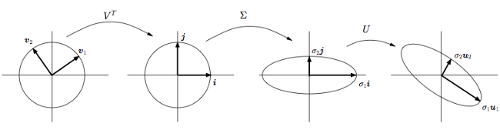
\includegraphics{linear_algebra_svd_illustration.png}
\end{center}

\begin{example}\label{} Consider the matrix $A = \left(\begin{array}{cc} 1 & 1 \\ 1 & 1 \\ 1 & -1 \end{array}\right)$. The matrix $A^tA = \left(\begin{array}{cc} 3 & 1\\ 1 & 3 \end{array}\right)$ has characteristic polynomial $\text{char}_{A^tA}(\lambda) = \lambda^2 - 6 \lambda + 8$ with eigenvalues $4$ and $2$ corresponding to orthonormal eigenvectors $v_1 = (\sqrt{2}/2, \sqrt{2}/2)$ and $v_2 = (\sqrt{2}/2, -\sqrt{2}/2)$. Hence $\sigma_1 = 2, \sigma_2 = \sqrt{2}$ and $u_1 = \sigma_1^{-1}Av_1 = (\sqrt{2}, \sqrt{2}, 0), u_2 = \sigma_2^{-1}Av_2 = (0, 0, \sqrt{2})$. If we add $u_3 = u_1 \times u_2$ to complete $u_1, u_2$ to an orthonormal basis then
$$\left(\begin{array}{cc} 1 & 1 \\ 1 & 1 \\ 1 & -1 \end{array}\right) = \left(\begin{array}{ccc} \sqrt{2}/2 & 0 & \sqrt{2}/2 \\ \sqrt{2}/2 & 0 & -\sqrt{2}/2 \\ 0 & 1 & 0 \end{array}\right) \left(\begin{array}{cc} 2 & 0 \\ 0 & \sqrt{2} \\ 0 & 0 \end{array}\right) \left(\begin{array}{cc} \sqrt{2}/2 & \sqrt{2}/2 \\ \sqrt{2}/2 & -\sqrt{2}/2 \end{array}\right)$$

We could use $u_3 = (-\sqrt{2}/2, \sqrt{2}/2)$ and the above equation would still hold, demonstrating the nonuniqueness of $U$ and as well of $V$ in general cases. Moreover, $\text{rank}(A) = \text{rank}(D) = r = 2$ while $\ker(A) = \{0\}$ and $\text{im}(A) = \text{Span}(v_1, v_2) \subsetneq \mathbb{R}^3$.
\end{example}

\begin{example}\label{} Consider the total least squares problem of finding $w \in \mathbb{R}^n$ such that $||Aw||_2 = \text{min}\{||Av||_2, ||v||_2 = 1\}$ for any matrix $A \in M(m, n, \mathbb{R})$. The solution turns out to be the right singular vector of $A$ corresponding to the smallest singular value. One can find other applications of singular value decomposition to data compression and principal component analysis in various fields.
\end{example}

\begin{exercise}\label{} Reconsider the wide matrix $A = \left(\begin{array}{ccc} 2 & 1 & 1 \\ 1 & 2 & 1 \end{array}\right)$ in example \ref{rightinvertible}.
\begin{enumerate}[\indent a.]
\item Compute the characteristic polynomial, eigenvalues and orthonormal eigenvectors for $AA^t$.
\item Compute the characteristic polynomial, eigenvalues and orthonormal eigenvectors for $A^tA$.
\item Compute the singular values and orthonormal left singular vectors.
\item Compute the singular value decomposition.
\item Use this decomposition to compute right inverse for $A$ and compare with previous result. This is the second way to find right inverse of a right invertible matrix.
\end{enumerate}
\end{exercise}

\part{Matrix Algorithms}\label{matrixalgorithms}  Linear algebra has extensive applications in many modern disciplines, especially those that work with data in Euclidean spaces. One major application is to solve a system of equations
$$a_{11}x_1 + \ldots + a_{1n}x_n = b_1$$
$$\vdots$$
$$a_{m1}x_1 + \ldots + a_{mn}x_n = b_m$$
where $a_{ij}, b_i \in F$. If we view $A = (a_{ij}) \in M(m, n,F)$ as a linear map $F^n \rTo^A F^m$ then we are looking to find solution $x = (x_1, \dots, x_n) \in F^n$ such that $Ax = b$ where $b = (b_1, \dots , b_m) \in F^m$. Below are some of the scenarios, but not all.
\begin{enumerate}[\indent i.]
\item for each $b \in F^m$ there are infinitely many solutions. This means $m < n$ and $A$ is right invertible with full image.
\item for each $b \in F^m$ there is a unique solution. This means $m = n$ and $A$ is invertible.
\item for some $b \in F^m$ there is no solution. This means $im(A) \subsetneq F^m$. The reason may be $m > n$ even though $A$ is left invertible with trivial kernel. Or it may be $m \leq n$ but $\text{rank}(A) < m \leq n$ and $A$ is not left invertible.
\end{enumerate}

\section{Complexity of Matrix Algorithms} As engineers, you devise efficient ways to solve such systems of equations when $A$ falls into one of these scenarios. You also care about the cost to solve them. 
\dfn A flop is an execution of either $+$ or $\cdot$ in $F$.

To evaluate the complexity of an algorithm, we write the total number of flops in that algorithm as a function of the sizes of objects at hand, for example $f(m, n)$ for matrices $A \in M(m, n,F)$, and simplify the expression by discarding minor terms. Flop count played a larger role when flops were slow and their count gave an accurate prediction of time cost. Nowadays that is no longer the case and flop count gives a rough estimate of time cost, especially when we consider its order.

\begin{example} Taking inner product $\langle (x_1, \dots, x_n), (y_1, \dots, y_n)\rangle$ takes $n$ multiplications and $n-1$ additions for $2n-1$ flops. We only keep $f(n) = 2n$ as a polynomial of the size $n$ of our vectors.
\end{example}

\begin{example} Adding $A, B \in M(m, n,F)$ takes $mn$ additions for $mn$ flops. We keep $f(m, n) = mn$ as a polynomial of the size of our matrices.
\end{example}

\begin{example} If $A \in M(m, n,F)$ and $x \in F^n$ then computing $Ax$ takes $m$ inner products, hence $m(2n-1)$ flops. We keep $f(m, n) = 2mn$. In case $A \in M(n, F)$ is diagonal then computing $Ax$ takes only $n$ flops. In another case $A = BC$ where $B \in M(m,p,F)$ and $C \in M(p, n, F)$ then computing $Ax = BCx$ takes $2pn + 2mp = 2p(m + n)$ flops, much few than $2mn$ when $p \ll \text{min}\{m, n\}$.
\end{example}

\begin{example} Multiplying two matrices $A \in M(m, n,F), B \in M(n, p, F)$ takes $mn$ inner products of vectors of size $n$ for $mp(2n-1)$ flops, or $2mnp$ if $n \gg 1$. In case $m = p$ and $AB$ is symmetric, this number decreases to $(m^2/2 + m)(2n -1) = m(m+1)(2n-1)/2$, or $m^2n$ as the leading term. Flop count in multiplying more than two matrices depends on how we parse the product. For $A \in M(m, n,F), B \in M(n,p,F), C \in M(p,q,F)$, computing $(AB)C$ takes $2mp(n+q)$ flops while computing $A(BC)$ takes $2nq(m+p)$ flops. The first computation is better when $2mp(n+q) < 2nq(m+p)$, i.e. when $1/n + 1/q < 1/m + 1/p$.
\end{example}

\begin{example} Consider the system $Ax = b$ where $A \in M(n, F)$ is triangular. Assume $A$ is lower triangular.
$$\left(\begin{array}{cccc} a_{11} & 0 & \dots & 0 \\ a_{21} & a_{22} & \dots & 0 \\ \vdots & \vdots & . & \vdots \\ a_{n1} & a_{n2} & \dots & a_{nn} \end{array}\right)\left(\begin{array}{c} x_1 \\ x_2 \\ \vdots \\ x_n \end{array}\right) = \left(\begin{array}{c} b_1 \\ b_2 \\ \vdots \\ b_n \end{array}\right) $$

Surely $x_1 = b_1/a_{11}, x_2 = (b_2 - a_{21}x_1)/a_{22}, x_3 = (b_3 - a_{31}x_1 - a_{32}x_2)/a_{33}1, \dots, x_n = (b_n - a_{n1}x_1 - a_{n2}x_2 - \ldots - a_{n(n-1)}x_{n-1})/a_nn$, each step taking $1, 3, 5, \dots ,(2n-1)$ flops for a total of $n^2$ flops. This algorithm is called forward substitution. If $A$ is diagonal then there are only $n$ divisions, so the algorithm take $n$ flops. Or if $A$ is sparse with at most $k$ nonzeros in each row then each substitution step takes $2k -1$ flops and the algorithm takes $2(k -1)n \approx 2kn$ flops. If $A$ is upper triangular, the algorithm is called backward substitution and works in a transposed fashion. Whether we get through all the substitution steps, i.e. whether $Ax = b$ is solvable depends on the innate properties of $A$. By corollary \ref{invertibletriangularmatrix}, the system has unique solution iff $A$ is invertible iff all its diagonal entries are nonzero. If we write $A^{-1} = \left(\begin{array}{ccc} x_1 & \dots & x_n \end{array}\right)$ in that case then $AA^{-1} = I$ sets up $n$ systems of linear equations $Ax_1 = e_1, \dots , Ax_n = e_n$. We can perform either algorithm above to solve each equation for $x_i$ and get $A^{-1}$.
\end{example}

\section{Cholesky Decomposition} We consider solving a system of equations $Ax = b$ where $A \in M(n, \mathbb{R})$ is positive definite.

\begin{theorem}\label{} (Cholesky Decomposition) Every positive semidefinite matrix $A \in M(n, \mathbb{R})$ can be decomposed as $A = LL^t$ where $L \in L(n, \mathbb{R})$ is lower triangular.
\end{theorem}
\begin{proof} By theorem \ref{LDUdecomposition}, $A = L'DL'^t = L'BBL'^t = L'BB^tL'^t = (L'B)(L'B)^t = LL^t$ where $B = \sqrt{D}$ is triangular and $L,L'$ are lower triangular.
\end{proof}

This Cholesky decomposition is unique for positive definite matrices and this is their form as a Gram matrix, recall \ref{Grammatrixpositivesemidefinite}. All matrices involved are then invertible. Again we do not claim $L$ to be orthogonal, otherwise we would have $L^t = L^{-1}$ above.

\begin{example} Positive semidefinite $A = (a_1, \dots , a_n) \in M(n, F)$ with nonnegative $a_i$ has Cholesky decomposition $(\sqrt{a_1}, \dots, \sqrt{a_n})(\sqrt{a_1}, \dots, \sqrt{a_n})$. When $A$ has some zero $a_i$ then perhaps we can find another decomposition, showing nonuniqueness. 
\end{example}

\begin{example}\label{} Positive definite $\left(\begin{array}{cc} 4 & 2 \\ 2 & 10 \end{array}\right)$ has unique Cholesky decomposition $\left(\begin{array}{cc} 2 & 0 \\ 1 & 3 \end{array}\right)\left(\begin{array}{cc} 2 & 1 \\ 0 & 3 \end{array}\right)$.
\end{example}

We will return to how Cholesky decomposition works and how it takes $n^3/3$ flops. Meanwhile, let's see what it does for us. Suppose we had to solve a system of linear equations $Ax = b$ where $A$ is positive definite. If we write $Ax = LL^tx = Ly = b$ then we see,
\begin{itemize}
\item Cholesky decomposition takes $n^3/3$ flops.
\item Solving $Ly = b, L$ lower triangular takes $n^2$ flops.
\item Solving $L^tx = y, L$ upper triangular takes $n^2$ flops.
\item Hence the total cost is $n^3/3 + 2n^2 \approx n^3/3$ flops.
\end{itemize}

\begin{example} Suppose we had to solve $4x_1 + 2x_2 = 3, 2x_1 + 10x_2 = 5$. Factoring $\left(\begin{array}{cc} 4 & 2 \\ 2 & 10 \end{array}\right)$ into $\left(\begin{array}{cc} 2 & 0 \\ 1 & 3 \end{array}\right)\left(\begin{array}{cc} 2 & 1 \\ 0 & 3 \end{array}\right)$ takes $2^3/3$ flops. Solving $\left(\begin{array}{cc} 2 & 0 \\ 1 & 3 \end{array}\right)\left(\begin{array}{c} y_1 \\ y_2 \end{array}\right) = \left(\begin{array}{c} 3 \\ 5 \end{array}\right)$ to get $(y_1, y_2) = (3/2,7/6)$ takes $2^2$ flops. Lastly solving $\left(\begin{array}{cc} 2 & 1 \\ 0 & 3 \end{array}\right)\left(\begin{array}{c} x_1 \\ x_2 \end{array}\right) = \left(\begin{array}{c} 3/2 \\ 7/6 \end{array}\right)$ to get $(x_1, x_2) = (5/9,7/18)$ takes another $2^2$ flops. The total cost is $8/3 + 2 \cdot 2^2$ flops.
\end{example}

Suppose we had to solve multiple systems $Ax_1 = b_1, \dots , Ax_m = b_m$, which is equivalent to solving the matrix equation $A_{n \times n}X_{n \times m} = B_{n \times m}$ where $X$ has $i^{\text{th}}$ column $x_i$ and $B$ has $j^{\text{th}}$ column $b_j$. Of course we don't repeat Cholesky decomposition, so the total flop count is $n^3/3 + 2mn^2$. The effort of solving a small number of systems with the same $A$ is roughly the effort of solving one system. This applies to finding the inverse of $A$, i.e. finding $X$ such that $AX = I$ since we know any positive definite matrix $A = LL^t$ is invertible by corollary \ref{positivedefiniteAtrivialkernelA^tfullimage} with inverse $A^{-1} = (L^t)^{-1}L^{-1} = (L^{-1})^tL^{-1}$. The cost for $A^{-1}$ is then $n^3/3 + 2n \cdot n^2 = 7n^3/3$. Is this cheaper than finding $L^{-1}$ and multiplying with $(L^{-1})^t$?

We can also prove existence of Cholesky decomposition for positive definite matrix $A = LL^t$ by recursion, starting with the partition
$$\left(\begin{array}{cc} a_{11} & A^t_{21} \\ A_{21} & A_{22} \end{array}\right) = \left(\begin{array}{cc} l_{11} & 0 \\ L_{21} & L_{22} \end{array}\right) \left(\begin{array}{cc} l_{11} & L^t_{21} \\ 0 & L^t_{22} \end{array}\right) = \left(\begin{array}{cc} l^2_{11} & l_{11}L^t_{21} \\ l_{11}L_{21} & L_{21}L^t_{21} + L_{22}L^t_{22} \end{array}\right)$$

Hence $l_{11} = \sqrt{a_{11}}, L_{21} = \frac{1}{l_{11}}A_{21}$, and $L_{22}L^t_{22} = A_{22} - L_{21}L^t_{21}$. This means we now must find $L_{22}$ in Cholesky decomposition of the positive definite matrix $A_{22} - L_{21}L^t_{21} = A_{22} - \frac{1}{a_{11}}A_{21}A^t_{21}$ of smaller sizer $(n-1) \times (n-1)$. Eventually we arrive at Cholesky decomposition of a $1 \times 1$ matrix, which is just taking square root. As a process
\begin{enumerate}[\indent 1.]
\item Compute the first column of $l_{11} = \sqrt{a_{11}}$ and $L_{21} = \frac{1}{l_{11}}A_{21}$ of $L$.
\item Compute Cholesky decomposition $A_{22} - L_{21}L_{21}^t = L_{22}L_{22}^t$.
\end{enumerate}

The whole algorithm takes $n^3/3$ flops. It also verifies whether a matrix $A$ is positive definite, as it will stall at some recursive step with $a_{11} = 0$ if $A$ is not.

\begin{exercise}\label{} Perform Cholesky decomposition for $\left(\begin{array}{ccc} 2 & -1 & 0 \\ -1 & 2 & -1 \\ 0 & -1 & 2 \end{array}\right)$.
\end{exercise}

\section{LU Decomposition} Next, we consider solving $Ax = b$ where $A \in M(n, \mathbb{R})$ is invertible, using the same factor-solve approach as in the previous subsection. Suppose we can factor $A = A_1 \dots A_k$ where each $A_i$ is special and $k$ is small in $f$ flops. Then we can solve $A_1x_1 = b, A_2x_2 = x_1, \dots , A_kx = x_{k-1}$ sequentially in $g$ flops. The total flop count is $f+g \approx f$ when $f$ is dominant.

\begin{example} Solving $Ax = b$ where $A \in M(n, \mathbb{R})$ is positive definite costs $n^2/3 + 2n^2$ flops.
\end{example}

Again this approach is effective in solving $m$ systems of equations sharing the same coefficient matrix $A$, as the cost is then $f + mg \approx f$ when $f$ is dominant. We look at the existence of such decomposition.

\begin{theorem}\label{LUdecomposition} (LU Decomposition for Invertible Matrices) Every invertible matrix $A \in M(n, \mathbb{R})$ can be decomposed as $A = PLU$ where $P \in M(n, \mathbb{R})$ is permuting, $L \in L(n, \mathbb{R})$ is unit lower triangular and $U \in U(n, \mathbb{R})$ is upper triangular.
\end{theorem}
\begin{proof} use theorem \ref{eigenvaluedecomposition}.
\end{proof}

\begin{example}\label{LUdecompositionexample1} $\left(\begin{array}{ccc} 2 & 1 & 3\\ 0 & 2 & 3 \\ 3 & 1 & 1 \end{array}\right) = \left(\begin{array}{ccc} 1 & 0 & 0\\ 0 & 0 & 1\\ 0 & 1 & 0 \end{array}\right)\left(\begin{array}{ccc} 1 & 0 & 0 \\ 3/2 & 1 & 0 \\ 0 & -4 & 1 \end{array}\right)\left(\begin{array}{ccc} 2 & 1 & 3 \\ 0 & -1/2 & -7/2 \\ 0 & 0 & -11 \end{array}\right)$. Wolframalpha will do this with command ``LU decomposition".
\end{example}

Here is the explicit algorithm to solve a system $Ax = b$ for invertible $A \in M(n, \mathbb{R})$.
\begin{enumerate}[\indent 1.]
\item Factoring $A = PLU$ in $2n^3/3$ flops.
\item Computing $z = P^tb$ where $Pz = b$ in 0 flop.
\item Forward substituting for $Ly = z$ in $n^2$ flops.
\item Backward substituting for $Ux = y$ in $n^2$ flops.
\end{enumerate}

Total cost is $2n^3/3 + 2n^2 \approx 2n^3/3$ flops. This is the standard method in the industry.

\begin{example}\label{LUdecompositionexample2} Given a system $2x_1 + x_2 + 3x_3 = 4, 0x_1 + 2x_2 + 3x_3 = 2, 3x_1 + x_2 + x_3 = 1$ we form $A$ as in example \ref{LUdecompositionexample1} and get its decomposition. Next we calculate
$$\left(\begin{array}{ccc} 1 & 0 & 0\\ 0 & 0 & 1\\ 0 & 1 & 0 \end{array}\right)\left(\begin{array}{c} z_1 \\ z_2 \\ z_3 \end{array}\right) = \left(\begin{array}{c} 4 \\ 2 \\1 \end{array}\right), \left(\begin{array}{c} z_1 \\ z_2 \\ z_3 \end{array}\right) = \left(\begin{array}{c} 4 \\ 1 \\ 2 \end{array}\right)$$
$$\left(\begin{array}{ccc} 1 & 0 & 0 \\ 3/2 & 1 & 0 \\ 0 & -4 & 1 \end{array}\right)\left(\begin{array}{c} y_1 \\ y_2 \\ y_3 \end{array}\right) = \left(\begin{array}{c} 4 \\ 1 \\ 2 \end{array}\right), \left(\begin{array}{c} y_1 \\ y_2 \\ y_3 \end{array}\right) = \left(\begin{array}{c} 4 \\ -5 \\-18 \end{array}\right)$$
$$\left(\begin{array}{ccc} 2 & 1 & 3 \\ 0 & -1/2 & -7/2 \\ 0 & 0 & -11 \end{array}\right)\left(\begin{array}{c} x_1 \\ x_2 \\ x_3 \end{array}\right) = \left(\begin{array}{c} 4 \\ -5 \\-18 \end{array}\right), \left(\begin{array}{c} x_1 \\ x_2 \\ x_3 \end{array}\right) = \left(\begin{array}{c} -24/11 \\ -16/11 \\ 18/11 \end{array}\right)$$
\end{example}

What step 2 actually does is follow $x= A^{-1}b = U^{-1}L^{-1}P^t b$. Moreover, solving multiple systems of $m$ equations with the same invertible coefficient matrix $A \in M(n, \mathbb{R})$  would cost $2n^3/3 + 2mn^2 \approx 2n^3/3$ flops if $n \gg m$. Lastly, solving for $A^{-1}$ is the same as solving $n$ systems $Ax_1 = e_1, \dots , Ax_n = e_n$ where $x_i$ is the $i^{\text{th}}$ column of $A^{-1}$. This would take $2n^3/3$ flops for LU decomposition plus $n \cdot 2n^2$ flops for $n$ forward substitutions and $n$ backward substitutions.

\subsection{LU Decomposition without Pivoting} We can also prove existence of LU decomposition for invertible matrix $A = PLU$ by recursion. Up first is the simple case $P = I$ and $A = LU$, which sets up a matrix equation in blocks,
$$\left(\begin{array}{cc} a_{11} & A_{12} \\ A_{21} & A_{22} \end{array}\right) = \left(\begin{array}{cc} 1 & 0 \\ L_{21} & L_{22} \end{array}\right)\left(\begin{array}{cc} u_{11} & U_{12} \\ 0 & U_{22} \end{array}\right)$$
where $L_{21} \in M(n-1,1, \mathbb{R}), U_{12} \in M(1, n-1, \mathbb{R})$, $L_{22} \in M(n-1, n-1, \mathbb{R})$ is unit lower triangular and $U_{22} \in M(n-1, n-1, \mathbb{R})$ is invertible upper triangular. This reduces the problem to LU decomposition for an $(n-1) \times (n-1)$ matrix $A_{22} - \frac{1}{a_{11}}A_{21}A_{12} = L_{22}U_{22}$. Repeat until we arrive at an $1 \times 1$ matrix, whose factors are square roots. This algorithm works only if $a_{11} \neq 0$ at each recursive step and no permutation is needed to permute a nonzero with $a_{11}$, hence the name no pivoting (or no permutation). Step by step
\begin{enumerate}[\indent 1.]
\item Calculate the first row of $u_{11} = a_{11}, U_{12} = A_{12}$ of $U$.
\item Calculate the first column $L_{21} = \frac{1}{a_{11}} A_{21}$ of $L$.
\item Factor $A_{22} - \frac{1}{a_{11}}A_{21}A_{12}$.
\end{enumerate}

\begin{example}\label{} Consider the invertible matrix $\left(\begin{array}{ccc} 4 & 3 & 2\\ 1 & 0 & 1\\ 2 & 3 & 4\end{array}\right)$.

In step 1
$$u_{11} = a_{11} = 4, U_{12} = A_{12} = \left(\begin{array}{cc} 3 & 2 \end{array}\right)$$

In step 2
$$L_{21} = \frac{1}{4}A_{12} = \frac{1}{4}\left(\begin{array}{c} 1 \\ 2 \end{array}\right) = \left(\begin{array}{c} 1/4 \\ 1/2 \end{array}\right)$$

In step 3
$$A_{22} - \frac{1}{4}A_{12}A_{21} = \left(\begin{array}{cc} 0 & 1\\ 3 & 4 \end{array}\right) - \frac{1}{4}\left(\begin{array}{c} 1 \\ 2 \end{array}\right)\left(\begin{array}{cc} 3 & 2 \end{array}\right) = \left(\begin{array}{cc} -3/4 & 1/2 \\ 3/2 & 3 \end{array}\right)$$
is invertible so we start over recursively.

Again
$$u_{11} = a_{11} = -\frac{3}{4}, U_{12} = A_{12} = \frac{1}{2}$$

Next
$$L_{21} = \frac{1}{a_{11}}A_{21} =  -\frac{4}{3}\frac{3}{2} = -2$$

Thirdly
$$A_{22} - \frac{1}{a_{11}}A_{21}A_{12} = 3 + \frac{4}{3}\frac{3}{2}\frac{1}{2} = 4 = 2\cdot 2$$

Now we put everything together
$$\left(\begin{array}{cc} -3/4 & 1/2 \\ 3/2 & 3 \end{array}\right) =  \left(\begin{array}{cc} 1 & 0 \\ -2 & 2 \end{array}\right) \left(\begin{array}{cc} -3/4 & 1/2 \\ 0 & 2 \end{array}\right) = L_{22}U_{22}$$
$$\left(\begin{array}{ccc} 4 & 3 & 2\\ 1 & 0 & 1\\ 2 & 3 & 4\end{array}\right) = \left(\begin{array}{ccc} 1 & 0 & 0 \\ 1/4 & 1 & 0 \\ 1/2 & -2 & 2 \end{array}\right)\left(\begin{array}{ccc} 4 & 3 & 2 \\ 0 & -3/4 & 1/2 \\ 0 & 0 & 2\end{array}\right) = LU$$.
\end{example}

\begin{example} The matrix $\left(\begin{array}{cc} 0 & -2\\ 1 & 1 \end{array}\right)$ can not be factored as $\left(\begin{array}{cc} 1 & 0 \\ l_{21} & 1 \end{array}\right)\left(\begin{array}{cc} u_{11} & u_{12} \\ 0 & u_{22} \end{array}\right)$ since the algorithm halts at first step with $a_{11} = 0$.
\end{example}

\subsection{Permutation Matrices} The above example shows that our algorithm will not start when $a_{11} = 0$. We must swap the first row with another row $i^{\text{th}}$ with nonzero $a_{i1}$ in order to proceed. The existence of such $a_{i1}$ is guaranteed by invertibility of $A$ and such movement does not change our solution. This can be done by a permutation matrix $P$. Let $\sigma \in S_n$ be a permutation of $\{1, \dots , n\}$. We can view it as a map $V \rTo^{\sigma} V, (x_1, \dots, x_n) \mapsto (x_{\sigma(1)}, \dots , x_{\sigma(n)})$. This map is linear with matrix representation $A_{\sigma} = (a_{ij})$ where $a_{ij} = 1$ if $\sigma(i) = j$ and $a_{ij} = 0$ otherwise.

\begin{example} If $\sigma = (1 3 2 4)$ then it maps $(x_1, x_2, x_3, x_4)$ to $(x_4, x_3, x_1, x_2)$ in $\mathbb{R}^4$ and
$$A_{\sigma} = \left(\begin{array}{cccc} 0 & 0 & 1 & 0 \\ 0 & 0 & 0 & 1 \\ 0 & 1 & 0 & 0 \\ 1 & 0 & 0 & 0 \end{array}\right)$$
\end{example}

If $\sigma^{-1}$ is the inverse of $\sigma$ as permutations then $\sigma^{-1}(j) = i$. As linear maps, $\sigma^{-1}$ is the inverse of $\sigma$ and $A_{\sigma^{-1}} = (a_{ji}) = A_{\sigma}^t = A_{\sigma}^{-1}$. That means solving a system $Ax = b$ where $A$ is a permutation matrix costs 0 flop, with $x = A^t b$.

\begin{exercise}\label{} Show that the map $V \rTo^{\sigma} V, (x_1, \dots, x_n) \mapsto (x_{\sigma(1)}, \dots , x_{\sigma(n)})$ is linear.
\end{exercise}

\begin{exercise}\label{} Given the permutation $\sigma = (1 \, 3 \, 4 \, 2) \in S_4$,
\begin{enumerate}[\indent a.]
\item Compute $\sigma(e_i)$ and its matrix representation $A_{\sigma}$ with respect to $\{e_1, \dots , e_4\}$.
\item Compute the inverse permutation $\sigma^{-1}$ and its matrix representation $A_{\sigma^{-1}}$.
\item Verify that $P_{\sigma^{-1}} = P_{\sigma}^t$ and $P_{\sigma} P_{\sigma^{-1}} = I$.
\item Compute $P_{\sigma} \left(\begin{array}{cccc} a_{11} & a_{12} & a_{13} & a_{14} \\ a_{21} & a_{22} & a_{23} & a_{24} \\ a_{31} & a_{32} & a_{33} & a_{34} \\ a_{41} & a_{42} & a_{43} & a_{44} \end{array} \right)$ to see how it permutes the rows.
\end{enumerate}
\end{exercise}

\subsection{LU Decomposition with Pivoting} We now describe an LU decomposition for invertible $A$ with possibly zero $a_{11}$ by induction. Any invertible $A = (a_{11}) \in M(1, \mathbb{R})$ can be written as $(1) (1)(a_{11})$. Suppose any invertible matrix $A \in M(n-1, \mathbb{R})$ has an LU decomposition. Consider invertible $A \in M(n, \mathbb{R})$. Since its first column is nonzero, there exists a permutation matrix $P^t_1$ such that $A' = P^t_1A = \left(\begin{array}{cc} a_{11}' & A_{12}' \\ A_{21}' & A_{22}' \end{array}\right)$ with $a_{11}' \neq 0$. The difference $A_{22}' - \frac{1}{a_{11}'}A_{21}'A_{12}'$ is called the Schur complement of $a_{11}'$ in $A'$. It is invertible of size $(n-1) \times (n-1)$ so it has a LU decomposition $P_2L_{22}U_{22}$ by induction. But then
\begin{align*}
A & = P_1A' \\
 & = P_1\left(\begin{array}{cc} a_{11}' & A_{12}' \\ A_{21}' & A_{22}' \end{array}\right) \\
 & = P_1\left(\begin{array}{cc} 1 & 0 \\ 0 & P_2 \end{array}\right)\left(\begin{array}{cc} a_{11}' & A_{12}' \\ P^t_2A_{21}' & P^t_2 A_{22}' \end{array}\right) \\
 & = P_1 \left(\begin{array}{cc} 1 & 0 \\ 0 & P_2  \end{array}\right)\left(\begin{array}{cc} a_{11}' & A_{12}' \\ P^t_2A_{21}' & L_{22}U_{22} + \frac{1}{a_{11}'} P^t_2 A_{21}' A_{12}'  \end{array}\right) \\
 & = P_1 \left(\begin{array}{cc} 1 & 0 \\ 0 & P_2  \end{array}\right) \left(\begin{array}{cc} 1 & 0 \\ \frac{1}{a_{11}'} P^t_2 A_{21}' & L_{22}  \end{array}\right)\left(\begin{array}{cc} a_{11}' & A_{12}' \\ 0 & U_{22}  \end{array}\right)
\end{align*}

We are done. Summarily, the algorithm takes $2n^3/3$ flops and runs as follows
\begin{enumerate}[\indent 1.]
\item Permute $A$ to $A'$ by a permutation matrix $P_1^t$ so that $a_{11}' \neq 0$.
\item Compute LU decomposition for $A_{22}' - \frac{1}{a_{11}'} A_{21}' A_{12}' = P_2L_{22}U_{22}$.
\item Put together $P = P_1 \left(\begin{array}{cc} 1 & 0 \\ 0 & P_2  \end{array}\right)$, $L = \left(\begin{array}{cc} 1 & 0 \\ \frac{1}{a_{11}'} P^t_2 A_{21}' & L_{22}  \end{array}\right)$ and $U = \left(\begin{array}{cc} a_{11}' & A_{12}' \\ 0 & U_{22} \end{array}\right)$.
\end{enumerate}

\begin{example} Consider the invertible matrix $A = \left(\begin{array}{ccc} 0 & 1 & 1\\ 1 & 1 & 2\\ 2 & 3 &3\end{array}\right)$.

In step 1, we permute it to $A' = \left(\begin{array}{ccc} 1 & 1 & 2 \\ 0 & 1 & 1\\ 2 & 3 & 3\end{array}\right)$ with $a_{11}' = 1$ by $P^t_1 = \left(\begin{array}{ccc} 0 & 1 & 0 \\ 1 & 0 & 0 \\ 0 & 0 &1 \end{array}\right)$.

In step 2, $A_{22}' - \frac{1}{a_{11}'} A_{21}' A_{12}' = \left(\begin{array}{cc} 1 & 1 \\ 3 & 3 \end{array}\right) - \frac{1}{1}\left(\begin{array}{c} 0 \\ 2 \end{array}\right)\left(\begin{array}{cc} 1 & 2 \end{array}\right) = \left(\begin{array}{cc} 1 & 1 \\ 1 & -1 \end{array}\right)$ is invertible so we start over recursively. This time $a_{11}' = 1$ is already nonzero so $P_2^t = I$.

Next $A_{22}' - \frac{1}{a_{11}'} A_{21}' A_{12}' = -1 - \frac{1}{1}\cdot 1 \cdot 1 = (1)(1)(-2)$.

So in step 3, $P_3 = 1, L_3 = 1$ and $U_3 = -2$.

Again in step 3, $P_2 = \left(\begin{array}{cc} 1 & 0 \\ 0 & 1 \end{array}\right), L_{22} = \left(\begin{array}{cc} 1 & 0 \\ 1 & 1 \end{array}\right)$ and $U_{22} = \left(\begin{array}{cc} 1 & 1 \\ 0 & -2 \end{array}\right)$.

Lastly $P = P_1\left(\begin{array}{cc} 1 & 0 \\ 0 & P_2 \end{array}\right) = \left(\begin{array}{ccc} 0 & 1 & 0 \\ 1 & 0 & 0 \\ 0 & 0 & 1 \end{array}\right)\left(\begin{array}{ccc} 1 & 0 & 0 \\ 0 & 1 & 0 \\ 0 & 0 &1 \end{array}\right) = \left(\begin{array}{ccc} 0 & 1 & 0 \\ 1 & 0 & 0 \\ 0 & 0 & 1 \end{array}\right)$, $L = \left(\begin{array}{cc} 1 & 0 \\ \frac{1}{a_{11}'} P^t_2 A_{21}' & L_{22}  \end{array}\right) = \left(\begin{array}{ccc} 1 & 0 & 0 \\ 0 & 1 & 0 \\ 2 & 1 & 1 \end{array}\right)$ and $ U = \left(\begin{array}{cc} a_{11}' & A_{12}' \\ 0 & U_{22} \end{array}\right) = \left(\begin{array}{ccc} 1 & 1 & 2 \\ 0 & 1 & 1\\ 0 & 0 & -2 \end{array}\right)$.
\end{example}

\begin{exercise}\label{} Perform LU decomposition for $\left(\begin{array}{ccc} 2 & -1 & 0 \\ -1 & 2 & -1 \\ 0 & -1 & 2 \end{array}\right)$.
\end{exercise}

\subsection{Effect of Rounding in Using LU Decomposition} We discuss the effect of rounding errors on the accuracy of the LU decomposition method for solving a system of linear equations. Consider the system $10^{-5}x_1 + x_2 = 1, x_1 + x_2 = 0$. Its exact solution is $(\frac{-1}{1 - 10^{-5}}, \frac{1}{1 - 10^{-5}})$. On the other hand, $A = \left(\begin{array}{cc} 10^{-5} & 1 \\ 1 & 1 \end{array}\right)$ has two LU decompositions
$$A = \left(\begin{array}{cc} 1 & 0 \\ 0 & 1 \end{array}\right)\left(\begin{array}{cc} 1 & 0 \\ 10^5 & 1 \end{array}\right)\left(\begin{array}{cc} 10^{-5} & 1 \\ 0 & 1 - 10^5 \end{array}\right)$$
$$A = \left(\begin{array}{cc} 0 & 1 \\ 1 & 0 \end{array}\right)\left(\begin{array}{cc} 1 & 0 \\ 10^{-5} & 1 \end{array}\right)\left(\begin{array}{cc} 1 & 1 \\ 0 & 1 - 10^{-5} \end{array}\right)$$

If we introduce some errors by rounding $a_{22} = 1 - 10^5 = -0.9999 \cdot 10^5$ in the first decomposition to four significant digits $-1.0000 \cdot 10^5 = -10^5$ and proceed to solve the system then we get solution $(0,1)$. The difference in result is huge. This phenomenon is called numerical instability and an algorithm is called numerically unstable if small errors along the way can cause significant error in the end. Solving linear equations using LU decomposition is numerically unstable.

Similarly, if we round $a_{22} = 1 - 10^{-5} = 0.99999$ in the second decomposition to 1 and solve the system then we get solution $(-1,1)$. In this case, the difference is tiny, $10^{-5}$ of the same order as the error we manufactured. This means choice of decomposition, i.e. choice of permutation matrix $P$, matters. Careful error analysis and extensive practical experience tell us to go with $P$ that permutes the entry of largest absolute value in the first column of $A$ to $a_{11}'$. Our example agrees with this.

\section{QR Decomposition} Now, we consider solving $Ax = b$ where $A \in M(m, n, \mathbb{R})$ is left invertible, again using the same factor-solve approach as in the previous two subsections. Recall the characterization of left invertible matrices in theorem \ref{onesidedinvertibility} and corollary \ref{leftinvertiblesquareortallrightinvertiblesquareorwide}.

\begin{theorem}\label{QRdecomposition} (QR Decomposition for Left Invertible Matrices) Every left invertible matrix $A \in M(m, n, \mathbb{R})$ can be decomposed as $A = QR$ where $Q \in M(m, n, \mathbb{R})$ is orthogonal with $Q^tQ = I_n$ and $R \in U(n, \mathbb{R})$ is upper triangular with positive diagonal entries.
\end{theorem}
\begin{proof} use theorem \ref{eigenvaluedecomposition}.
\end{proof}

The theorem only shows existence of $Q$ and $R$. Here is how to get them. If we partition $A, Q, R$ as
$$A = \left(\begin{array}{cc} a_1 & A_2 \end{array}\right) \hspace{30pt} Q = \left(\begin{array}{cc} q_1 & Q_2 \end{array}\right) \hspace{30pt} R = \left(\begin{array}{cc} r_{11} & R_{12} \\ 0 & R_{22} \end{array}\right)$$
then
\begin{align*}
\left(\begin{array}{cc} a_1 & A_2 \end{array}\right) & = \left(\begin{array}{cc} q_1 & Q_2 \end{array}\right) \left(\begin{array}{cc} r_{11} & R_{12} \\ 0 & R_{22} \end{array}\right)\\
 & = \left(\begin{array}{cc} q_1r_{11} & q_1R_{12} + Q_2R_{22} \end{array}\right)
\end{align*}
where $a_1 \in M(m, 1, \mathbb{R}), A_2 \in M(m, n-1, \mathbb{R}), q_1 \in M(m, 1, \mathbb{R}), Q_2 \in M(m, n-1, \mathbb{R}), r_{11} \in M(1, 1, \mathbb{R}), R_{12} \in M(1, n-1, \mathbb{R}), R_{22} \in M(n-1, n-1, \mathbb{R})$. For $Q$ to be orthogonal
\begin{align*}
Q^tQ & = \left(\begin{array}{c} q_1^t \\ Q_2^t \end{array}\right) \left(\begin{array}{cc} q_1 & Q_2 \end{array}\right) \\
 & = \left(\begin{array}{cc} q_1^tq_1 & q_1^tQ_2 \\ Q_2^tq_1 & Q_2^tQ_2 \end{array}\right) \\
 & = \left(\begin{array}{cc} 1 & 0 \\ 0 & 1 \end{array}\right)
\end{align*}
we must have $q_1^tq_1 = 1, q_1^tQ_2 = 0, Q_2^tQ_2 = I$. For $R$ to be upper triangular with positive diagonal entries, we must have $r_{11} > 0$ and $R_{22}$ is upper triangular with positive diagonal entries.

Putting things together, firsly we see $a_1 = q_1r_{11}$ so we choose $r_{11} = ||a_1||, q_1 = \frac{a_1}{r_{11}}$. Next we see $A_2 = q_1R_{12} + Q_2R_{22}$ which implies $q_1^tA_2 = q_1^tq_1R_{12} + q_1^tQ_2R_{22} = R_{12}$. So we compute $R_{12} = q_1^tA_2$. Lastly, we see $A_2 - q_1R_{12} = Q_2R_{22}$. This is QR decomposition of an $m \times (n-1)$ matrix. Continuing recursively, we arrive at QR decomposition of an $m \times 1$ matrix $A = QR$ where $Q = \frac{1}{||A||}A, R = ||A||$. This algorithm is called the modified Gram-Schmidt method. In summary, it runs
\begin{enumerate}[\indent 1.]
\item $r_{11} = ||a_1||$.
\item $q_1 = \frac{a_1}{r_{11}}$.
\item $R_{12} = q_1^t A_2$.
\item Compute QR decomposition $A_2 - q_1R_{12} = Q_2R_{22}$.
\end{enumerate} 

The total cost is $2mn^2$ flops. Note that $||a_1|| \neq 0$ in step 1 because $A$ has trivial kernel. Also $A_2 - q_1R_{12}$ is left invertible in step 4. Indeed, if $x \neq 0 \in \mathbb{R}^{n-1}$ then $(A_2 - q_1R_{12})x = A_2 x - \frac{a_1}{r_{11}}R_{12} x = (a_1 \,\,\, A_2)(- \frac{1}{r_{11}}R_{12}x \,\,\, x)^t = A(- \frac{1}{r_{11}}R_{12}x \,\,\, x)^t \neq 0$.

\begin{example}\label{QRdecompositionexample} The matrix $A = \left(\begin{array}{ccc} 3/5 & -6/5 & 26/5 \\ 4/5 & -8/5 & -7/5 \\ 0 & 4/5 & 4/5 \\ 0 & -3/5 & -3/5 \end{array} \right)$ has QR decomposition
$$\left(\begin{array}{ccc} 3/5 & 0 & 4/5 \\ 4/5 & 0 & -3/5 \\ 0 & 4/5 & 0 \\ 0 & -3/5 & 0 \end{array} \right) \left(\begin{array}{ccc} 1 & -2 & 2 \\ 0 & 1 & 1 \\ 0 & 0 & 5 \end{array} \right)$$
\end{example}

\begin{exercise}\label{} Perform QR decomposition for $\left(\begin{array}{ccc} 3 & 3 & 2 \\ 4 & 4 & 1\\ 0 & 6 & 2\\ 0 & 8 & 1 \end{array}\right)$
\end{exercise}

\section{Least Square Problem} If our system of equations $Ax = b$ falls into scenario $(ii)$ discussed at the beginning of part \ref{matrixalgorithms} then there is a unique $x$ such that $||Ax - b|| = 0$. If it falls into scenario $(iii)$ then $Ax \neq b$ and $||Ax - b|| > 0$ for all $x \in \mathbb{R}^n$ and we can only hope to find an $\hat{x}$ such that this nonzero norm is least. Either way, solving the system becomes minimization of
$$||Ax - b||^2 = \sum\limits_{i =1}^m (a_{i1}x_1 + \ldots + a_{in}x_n - b_i)^2 = \sum\limits_{i = 1}^m r_i(x)^2 \geq 0$$

This explains the name \textit{least square}. The word \textit{linear} is sometimes included to emphasize that each $r_i$ is linear in the $x_1, \dots, x_n$ plus a constant.

\begin{example}\label{} The system
$$ Ax = \left(\begin{array}{c} 1 \\ 0 \end{array}\right)(x) = \left(\begin{array}{c} 2 \\1 \end{array}\right)$$
has no solution. This is the embedding of $\mathbb{R}$ into $\mathbb{R}^2$ as the $x$-axis. By geometry, $\hat{x} = 2$ gives smallest $||Ax - b||$.
\end{example}

\begin{example}\label{} The system
$$Ax = \left(\begin{array}{cc} 2 & 0 \\ -1 & 1 \\ 0 & 2 \end{array} \right) \left(\begin{array}{c} x_1 \\ x_2 \end{array}\right) = \left(\begin{array}{c} 1 \\ 0 \\ -1 \end{array}\right)$$
has no solution. The corresponding least square problem is to minimize $f(x_1, x_2) = (2x_1 - 1)^2 + (-x_1 + x_2)^2 + (2x_2 + 1)^2$. Taking partial derivatives $\partial f / \partial x_1$ and $\partial f / \partial x_2$ yields solution $\hat{x} = (1/3, - 1/3)$ for minimum.
\end{example}

The following theorem tells us when we can expect existence and uniqueness of such $\hat{x}$.

\begin{theorem}\label{} If $A$ is a left invertible matrix then the least square problem for $Ax = b$ has unique solution $\hat{x} = (A^tA)^{-1}A^t b$.
\end{theorem}
\begin{proof} For $\hat{x} = (A^tA)^{-1}A^t b$ and any $x \in \mathbb{R}^n$, we show $||Ax - b||^2 = ||(Ax - A\hat{x}) + (A\hat{x} - b)||^2 = \langle (Ax - A\hat{x}) + (A\hat{x} - b), (Ax - A\hat{x}) + (A\hat{x} - b) \rangle =  ||Ax - A\hat{x}||^2 + ||A\hat{x} - b||^2 + 2(Ax - A\hat{x})^t(A\hat{x} - b) = ||A(x - \hat{x})||^2 + ||A\hat{x} - b||^2 + 0 \geq ||A\hat{x} - b||^2$. So $\hat{x}$ is solution to the least square problem. Uniqueness follows from the fact that equality holds iff $||A(x - \hat{x})|| = 0$ iff $A(x - \hat{x}) = 0$ iif $x - \hat{x} = 0$ iff $x = \hat{x}$.
\end{proof}

If $A$ is indeed invertible then $\hat{x} = (A^tA)^{-1}A^t b = A^{-1}(A^t)^{-1} A^t b = A^{-1} b$ the precise solution as we would expect. Else, $A^tA \hat{x} = A^tb$ still holds and so we are reduced to solving the system $A^tAx = A^tb$. It is called the system of normal equations associated with the least square problem for $Ax = b$.

\subsection{Cholesky Decomposition to Solve Least Square Problem} Since $A^tA$ is positive definite by theorem \ref{onesidedinvertibility}, we can apply Cholesky decomposition to solve the least square problem. An algorithm to do so runs as follows
\begin{enumerate}[\indent 1.]
\item Multiply $B = A^tA$ and $c = A^t b$.
\item Compute the Cholesky decomposition $B = LL^t$.
\item Solve $Ly = c$ by forward substitution.
\item Solve $L^tx = y$ by backward substitution.
\end{enumerate}

The cost to form $B = A^tA$ in step 1 is $mn^2$ flops, note that $B$ is symmetric so we only need to compute $n(n+1) / 2 \approx n^2 / 2$ elements in its lower triangle. The cost to calculate $c = A^t b$ is $2mn$. Step $2$ costs $n^3 / 3$ flops while step 3 and step 4 cost $n^2$ each. Hence the whole algorithm costs $mn^2 + n^3 / 3 + 2mn + 2n^2$ flops. Note that left invertibility implies $A$ is square or tall with $m \geq n$, so multiplication of $B = A^tA$ costs the most. If $m \gg n$ then the algorithm costs roughly $mn^2$ flops.

\begin{example}\label{leastsquareproblemCholeskydecompositionexample} Consider the system
$$Ax = \left(\begin{array}{ccc} 3/5 & -6/5 & 26/5 \\ 4/5 & -8/5 & -7/5 \\ 0 & 4/5 & 4/5 \\ 0 & -3/5 & -3/5 \end{array} \right)\left(\begin{array}{c} x_1 \\ x_2 \\ x_3 \end{array}\right) = \left(\begin{array}{c}1 \\ 1 \\ 1 \\ 1\end{array}\right)$$
where $A$ is from example \ref{QRdecompositionexample}. Then
$$B = A^tA = \left(\begin{array}{ccc} 1 & -1 & 2 \\ -2 & 5 & -3 \\ 2 & -3 & 30 \end{array}\right) = \left(\begin{array}{ccc} 1 & 0 & 0 \\ -2 & 1 & 0 \\ 2 & 1 & 5 \end{array}\right)\left(\begin{array}{ccc} 1 & -2 & 2 \\ 0 & 1 & 1 \\ 0 & 0 & 5 \end{array}\right)$$
in its Cholesky decomposition and $c = (7/5, -13/5, 4)$. It follows from there that $(y_1, y_2, y_3) = (7/5, 1/5, 1/5)$ by forward substitution and $(x_1, x_2, x_3) = (41/25, 4/25, 1/25)$ by backward substitution.
\end{example}

\begin{exercise}\label{leastsquareproblemCholeskydecompositionexercise} Consider the system
$$Ax = \left(\begin{array}{ccc} 1 & -1 & 4 \\ 1 & 4 & -2 \\ 1 & 4 & 2 \\ 1 & -1 & 0 \end{array}\right)\left(\begin{array}{c} x_1 \\ x_2 \\ x_3 \end{array}\right) = \left(\begin{array}{c}1 \\ 2 \\ 2 \\ 1\end{array}\right)$$
\begin{enumerate}[\indent a.]
\item Perform Cholesky decomposition for $A^tA$.
\item Use it to solve the least square problem for the above system.
\end{enumerate}
\end{exercise}

\subsection{QR Decomposition to Solve Least Square Problem} There is another way to solve the least square problem. By theorem \ref{QRdecomposition}, we can decompose left invertible $A = QR$ where $Q \in M(m, n, \mathbb{R})$ is orthogonal with $Q^tQ = I_n$ and $R \in U(n, \mathbb{R})$ is upper triangular with positive diagonal entries. Then $A^tA = (QR)^t(QR) = R^tQ^tQR = R^tR$ and $R^tRx = R^tQ^t b$. Since $R$ is invertible, this gives $Rx = Q^tb$. Packaged as an algorithm, it is
\begin{enumerate}[\indent 1.]
\item Compute the QR decomposition $A = QR$.
\item Compute $c = Q^tb$.
\item Solve $Rx = c$ by backward substitution.
\end{enumerate}

Step 1 costs $2mn^2$ flops while step 2 costs $2mn$ flops and step 3 costs $n^2$ flops. Total cost is $2mn^2 + 2mn + n^2$ flops. If $m \gg n$ then it is roughly $2mn^2$ flops and this method is slower than Cholesky method by a factor of about 2. However, it is more accurate.

\begin{example}\label{} Again consider the system in example \ref{leastsquareproblemCholeskydecompositionexample}.
$$Ax = \left(\begin{array}{ccc} 3/5 & -6/5 & 26/5 \\ 4/5 & -8/5 & -7/5 \\ 0 & 4/5 & 4/5 \\ 0 & -3/5 & -3/5 \end{array} \right)\left(\begin{array}{c} x_1 \\ x_2 \\ x_3 \end{array}\right) = \left(\begin{array}{c}1 \\ 1 \\ 1 \\ 1\end{array}\right)$$

By example \ref{QRdecompositionexample},
$$\left(\begin{array}{ccc} 3/5 & -6/5 & 26/5 \\ 4/5 & -8/5 & -7/5 \\ 0 & 4/5 & 4/5 \\ 0 & -3/5 & -3/5 \end{array} \right) = \left(\begin{array}{ccc} 3/5 & 0 & 4/5 \\ 4/5 & 0 & -3/5 \\ 0 & 4/5 & 0 \\ 0 & -3/5 & 0 \end{array} \right) \left(\begin{array}{ccc} 1 & -2 & 2 \\ 0 & 1 & 1 \\ 0 & 0 & 5 \end{array} \right)$$

So
$$c = Q^tb = \left(\begin{array}{cccc} 3/5 & 4/5 & 0 & 0 \\ 0 & 0 & 4/5 & -3/5 \\ 4/5 & -3/5 & 0 & 0 \end{array}\right)\left(\begin{array}{c} 1 \\ 1 \\ 1 \\ 1 \end{array}\right) = \left(\begin{array}{c} 7/5 \\ 1/5 \\ 1/5 \end{array}\right)$$

It follows from there that $(x_1, x_2, x_3) = (41/25, 4/25, 1/25)$.
\end{example}

\begin{exercise}\label{} Again consider the system in exercise \ref{leastsquareproblemCholeskydecompositionexercise}
$$Ax = \left(\begin{array}{ccc} 1 & -1 & 4 \\ 1 & 4 & -2 \\ 1 & 4 & 2 \\ 1 & -1 & 0 \end{array}\right)\left(\begin{array}{c} x_1 \\ x_2 \\ x_3 \end{array}\right) = \left(\begin{array}{c}1 \\ 2 \\ 2 \\ 1\end{array}\right)$$
\begin{enumerate}[\indent a.]
\item Perform QR decomposition for $A$.
\item Use it to solve the least square problem for the above system and compare with previous result.
\end{enumerate}
\end{exercise}

\section{Least Norm Problem} If our system falls into scenario $(i)$ at the beginning of part \ref{matrixalgorithms} then there are infinitely many solutions $x \in \mathbb{R}^n$ such that $||Ax - b|| = 0$. If it falls into scenario $(ii)$ then there is a unique $x$ such that $Ax = b$. Either way, we can ask which solution $\hat{x}$ has least norm.

\begin{example}\label{leastnormproblemexample1} The system
$$Ax = \left(\begin{array}{ccc} 1 & 0 & 0 \\ 0 & 1 & 0 \end{array}\right)\left(\begin{array}{c} x_1 \\ x_2 \\ x_3 \end{array}\right) = \left(\begin{array}{c} 2 \\ 1 \end{array}\right)$$
has infinitely many solutions $(2,1, t), t \in \mathbb{R}$. This is the projection of $\mathbb{R}^3$ into its $xy$-plane. By geometry, $\hat{x} = (2,1,0)$ has smallest norm.
\end{example}

\begin{example}\label{leastnormproblemexample2} The system
$$Ax = \left(\begin{array}{ccc} 1 & -1 & 2 \\ 1 & 1 & -1 \end{array}\right) \left(\begin{array}{c} x_1 \\ x_2 \\ x_3 \end{array}\right) = \left(\begin{array}{c} 1 \\ 0 \end{array}\right)$$
has infinitely many solutions. The corresponding least norm problem is to minimize $f(x_1, x_2, x_3) = x_1^2 + x_2^2 + x_3^2$ subject to relations $x_1 - x_2 + 2x_3 = 1$ and $x_1 + x_2 - x_3 = 0$. We gather information $x_3 = x_1 + x_2$ and $x_2 = 1 - 3x_1$. Hence we need to minimize $f(x_1) = x_1^2 + (1-3x_1)^2 + (1-2x_1)^2$. Taking derivative yields solution $\hat{x} = (5/14, -1/14, 2/7)$ for minimum.
\end{example}

The following theorem tells us when we can expect existence and uniqueness of such $\hat{x}$.

\begin{theorem}\label{} If $A$ is a right invertible matrix then the least norm problem for $Ax = b$ has unique solution $\hat{x} = A^t(AA^t)^{-1} b$.
\end{theorem}
\begin{proof} Surely $A\hat{x} = AA^t(AA^t)^{-1}b = b$. And if $x$ is another solution to $Ax = b$ then $||x||^2 = ||(x - \hat{x}) + \hat{x}||^2 = ||x - \hat{x}||^2 + ||\hat{x}||^2 + 2\hat{x}^t(x - \hat{x}) = ||x - \hat{x}||^2 + ||\hat{x}||^2 + 0 \geq ||\hat{x}||^2$ because $\hat{x}^t(x - \hat{x}) = (A^t(AA^t)^{-1}b)^t(x - \hat{x}) = b^t(AA^t)^{-1}A(x-\hat{x}) = b^t(AA^t)^{-1}(b-b) = 0$. Uniqueness follows from the fact that equality holds iff $||x - \hat{x}|| = 0$ iff $x - \hat{x} = 0$ iff $x = \hat{x}$.
\end{proof}

If $A$ is indeed invertible then $\hat{x} = A^t(AA^t)^{-1} b = A^t(A^t)^{-1} A^{-1} b = A^{-1} b$ the precise solution as we would expect. Else, we can still solve $AA^t z = b$ and $\hat{x} = A^t z$. The first equality is called the system of normal equations associated with the least norm problem for $Ax = b$.

\subsection{Cholesky Decomposition to Solve Least Norm Problem} Since $AA^t$ is also positive definite by theorem \ref{onesidedinvertibility}, we can apply Cholesky decomposition to solve the least norm problem. An algorithm to do so runs as follows.
\begin{enumerate}[\indent 1.]
\item Multiply $B = AA^t$.
\item Compute the Cholesky decomposition $B = LL^t$.
\item Solve $Lz = b$ by forward substitution.
\item Solve $L^t y = z$ by backward substitution.
\item Compute $x = A^ty$.
\end{enumerate}

The cost to form $B = A^tA$ in step 1 is $m^2n$, note again that $B$ is symmetric. Steps 2, 3, 4, 5 cost $m^3/3, m^2, m^2, 2mn$ flops. Hence the whole algorithm costs $m^2n + m^3/3 + 2m^2 + 2mn$ flops. Note that right invertibility implies that $A$ is square or wide with $m \leq n$, so again multiplication of $B = AA^t$ costs the most. If $m \ll n$ then the algorithm costs roughly $m^2n$ flops.

\begin{example}\label{leastsnormproblemCholeskydecompositionexample} Consider the system
$$Ax = \left(\begin{array}{cccc} 1 & -1 & 1 & 1 \\ 1 & 0 & 1/2 & 1/2 \end{array} \right)\left(\begin{array}{c} x_1 \\ x_2 \\ x_3 \\ x_4 \end{array}\right) = \left(\begin{array}{c} 0 \\ 1\end{array}\right)$$

Then
$$B = AA^t = \left(\begin{array}{cc} 2 & 0 \\ 1 & 1/ \sqrt{2} \end{array}\right) \left(\begin{array}{cc} 2 & 1 \\ 0 & 1/ \sqrt{2} \end{array}\right)$$

It follows from there that $(z_1, z_2) = (0, \sqrt{x})$ by forward substitution and $(y_1, y_2) = (-1,2)$ by backward substitution. Finally, $(x_1, x_2) = A^t(y_1, y_2) = (1,1,0,0)$.
\end{example}

\begin{exercise}\label{leastnormproblemCholeskydecompositionexercise} Consider the system in example \ref{leastnormproblemexample2}.
$$Ax = \left(\begin{array}{ccc} 1 & -1 & 2 \\ 1 & 1 & -1 \end{array}\right) \left(\begin{array}{c} x_1 \\ x_2 \\ x_3 \end{array}\right) = \left(\begin{array}{c} 1 \\ 0 \end{array}\right)$$
\begin{enumerate}[\indent a.]
\item Perform Cholesky decomposition for $AA^t$.
\item Use it to solve the least norm problem for the above system and compare with previous result.
\end{enumerate}
\end{exercise}

\subsection{QR Decomposition to Solve Least Norm Problem} There is another way to solve the least norm problem. By theorem \ref{QRdecomposition}, we can decompose $A^t = QR$ where $Q \in M(n, m, \mathbb{R})$ is orthogonal with $Q^tQ = I_m$ and $R \in M(m, \mathbb{R})$ is upper triangular with positive diagonal entries. Then $\hat{x} = A^t(AA^t)^{-1}b = QR(R^tQ^tQR)^{-1}b = QR(R^tR)^{-1}b = QRR^{-1}(R^t)^{-1}b = Q(R^t)^{-1}b$. Packaged as an algorithm, it is
\begin{enumerate}[\indent 1.]
\item Compute the QR decomposition $A^t = QR$.
\item Solve $R^ty = b$ by forward substitution.
\item Compute $x = Qy$.
\end{enumerate}

Step 1 costs $2nm^2$ flops while step 2 costs $m^2$ flops and step 3 costs $2mn$ flops. Total cost is $2m^2n + m^2 + 2mn$ flops. If $m \ll n$ then it is roughly $2m^2n$ flops and this method is slower than the Cholesky method by a factor of about 2. However, it is more accurate.

\begin{example}\label{leastsnormproblemQRdecompositionexample} Again consider the system in example \ref{leastsnormproblemCholeskydecompositionexample}.
$$Ax = \left(\begin{array}{cccc} 1 & -1 & 1 & 1 \\ 1 & 0 & 1/2 & 1/2 \end{array} \right)\left(\begin{array}{c} x_1 \\ x_2 \\ x_3 \\ x_4 \end{array}\right) = \left(\begin{array}{c} 0 \\ 1\end{array}\right)$$

The $QR$ factorization for $A^t$ is
$$\left(\begin{array}{cc} 1 & 1 \\ -1 & 0 \\ 1 & 1/2 \\ 1 & 1/2 \end{array}\right) = \left(\begin{array}{cc} 1/2 & 1/ \sqrt{2} \\ -1/2 & 1/ \sqrt{2} \\ 1/2 & 0 \\ 1/2 & 0 \end{array}\right) \left(\begin{array}{cc} 2 & 1 \\ 0 & 1/ \sqrt{2} \end{array}\right)$$

It follows from there that $(y_1, y_2) = (0, \sqrt{2})$ and $(x_1, x_2, x_3, x_4) = (1,1,0,0)$.
\end{example}

\begin{exercise}\label{leastsnormproblemQRdecompositionexercise} Again consider the system in exercise \ref{leastnormproblemCholeskydecompositionexercise}.
$$Ax = \left(\begin{array}{ccc} 1 & -1 & 2 \\ 1 & 1 & -1 \end{array}\right) \left(\begin{array}{c} x_1 \\ x_2 \\ x_3 \end{array}\right) = \left(\begin{array}{c} 1 \\ 0 \end{array}\right)$$
\begin{enumerate}[\indent a.]
\item Perform QR decomposition for $A^t$.
\item Use it to solve the least norm problem for the above system and compare with previous result.
\end{enumerate}
\end{exercise}

\center{\textit{to Aaron Swartz and a free open internet}.}

\end{document}